% Requires packages: graphicx, booktabs, tabularx
\chapter{Background and Related Work}
\label{ch:background}

This chapter provides the shared foundations for the dissertation. It serves two purposes. The first three sections are introductory. They operationalise the objects and coordinates that recur across the later chapters: musical dynamics, perceived loudness in audio, and dynamics in MIDI and score. The remaining sections form a literature review aligned with the three thesis contribution lines and the data conditions under which they operate.

Section~\ref{sec:bg:dynamics} operationalises musical dynamics across physical sound level, perceived loudness, MIDI velocity, and score-level symbols. Section~\ref{sec:bg:dynamics:audio} introduces loudness-oriented audio representations. Section~\ref{sec:bg:dynamics_midi_score} covers symbolic dynamics in MIDI and score, including alignment and representation choices that determine what supervision actually means. Section~\ref{sec:bg:expressive_mir} then turns to the expressive-MIR landscape: it sketches the historical trajectory from performance research to deep-learning AMT and identifies the three task lines that anchor the thesis. Sections~\ref{sec:bg:velocity} and~\ref{sec:bg:scoredyn} review the first two of these literatures in depth: note-level MIDI velocity recovery and beat-synchronous score-dynamics recovery. Section~\ref{sec:bg:synthesis} reviews the third: traditional and differentiable audio synthesis as it relates to dynamics, including the analysis-by-synthesis route to label-scarce velocity recovery. Section~\ref{sec:bg:dataeval} surveys the datasets and evaluation conventions that constrain what each chapter can claim. The chapter ends by converting the literature gaps into explicit thesis requirements.

\section{Musical Dynamics}
\label{sec:bg:dynamics}

The word \emph{dynamics} is used in several related but non-identical ways across music theory, performance research, and MIR. That distinction is not a terminological luxury. It determines what target is being estimated, what evidence is relevant, and what evaluation is legitimate. Figure~\ref{fig:bg_dynamics_layers} provides the layered view of dynamics used throughout this thesis.

\begin{figure}[!htbp]
  \centering
  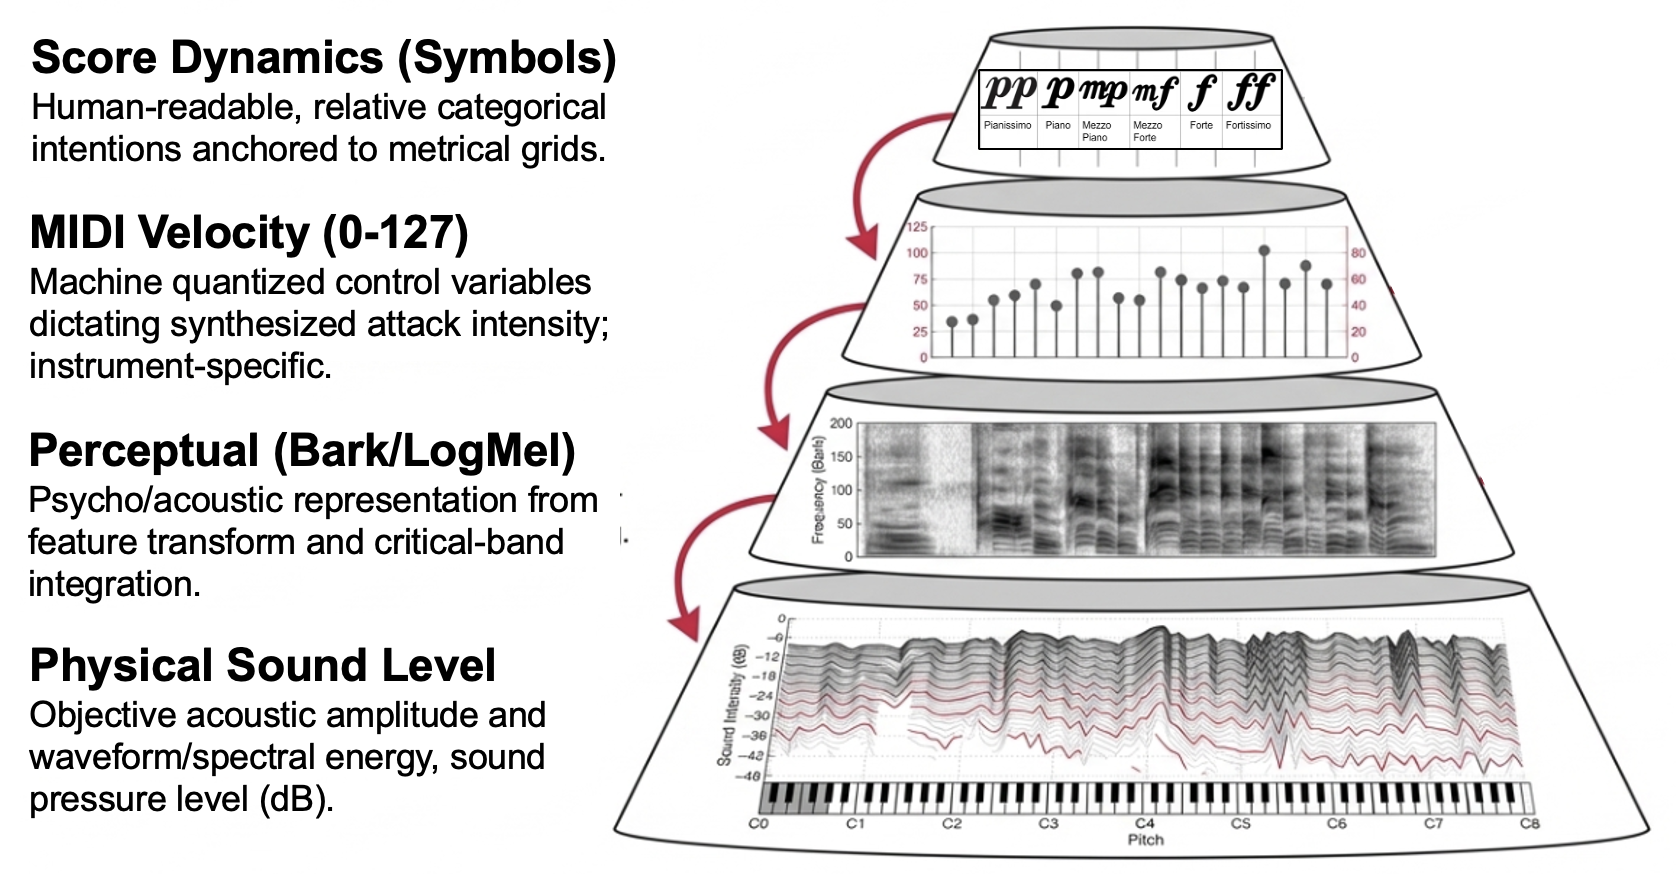
\includegraphics[width=0.9\linewidth]{Chapter_2/figures/dynamics_layers_v1.jpg}
  \caption{Layered view of dynamics used in this thesis. Physical sound level, perceived loudness, MIDI velocity, and score dynamics are linked but not interchangeable. Each transition is many-to-many or instrument-specific.}
  \label{fig:bg_dynamics_layers}
\end{figure}

\subsection{From physical sound level to symbolic dynamics}
\label{sec:bg:dynamics:layers}

A useful starting distinction is between \emph{physical intensity}, \emph{perceived loudness}, \emph{performance control}, and \emph{score notation}. Physical measurements such as sound-pressure level in decibels describe the signal. Human listeners do not hear decibels directly. They hear loudness, which depends on frequency content, masking, and temporal integration \cite{zwicker2007psychoacoustics,zwicker1999psychoacoustics}. MIDI velocity describes a control quantity at note onset. In acoustic piano settings it is best interpreted as a proxy for performer action rather than as a universal loudness unit \cite{goebl2003role,dan2006psy}. Score dynamics such as \textit{pp}, \textit{mf}, \textit{f}, or a hairpin do something else again. They encode relative musical intention in context \cite{kosta2014dynpiano,kosta2016mapping}.

This layered view has an important methodological consequence. There is no single exact lookup table that converts score dynamics, loudness, and MIDI velocity into one another. Nominal mappings are convenient for notation software and rendering systems, but they remain conventions. They should not be mistaken for measurement standards. This point is central to the whole dissertation because each chapter targets a different layer of the same broader expressive problem. Table~\ref{tab:bg_dynamics_compare} summarises the three dynamics representations that recur throughout this thesis, together with their temporal anchors, strengths, and limitations.

\begin{table}[!htbp]
\centering
\caption{Three dynamics representations that recur throughout this thesis.}
\label{tab:bg_dynamics_compare}
\small
\setlength{\tabcolsep}{4pt}
\renewcommand{\arraystretch}{1.18}
\begin{tabularx}{\textwidth}{
>{\raggedright\arraybackslash}p{0.20\textwidth}
>{\raggedright\arraybackslash}p{0.18\textwidth}
>{\hsize=0.92\hsize\raggedright\arraybackslash}X
>{\hsize=1.08\hsize\raggedright\arraybackslash}X
}
\toprule
\textbf{Representation} & \textbf{Temporal anchor} & \textbf{Main strength} & \textbf{Main limitation} \\
\midrule
Audio loudness & frame-wise / continuous & Closest to what is directly observable from audio about perceived intensity & Entangled with timbre, pitch, room acoustics, the recording chain, and instrument-specific response \\
MIDI velocity & note onset & Precise, machine-readable, and editable in symbolic performance workflows & Acts as a control proxy, not a universal loudness scale; not directly comparable across instruments or renderers \\
Score dynamics & beat / phrase level & Human-readable, interpretable, and naturally attached to score structure & Relative, sparse, context-dependent, and expensive to verify at scale \\
\bottomrule
\end{tabularx}
\end{table}


\subsection{Dynamics Roles in Music Performance}
\label{sec:bg:dynamics:musical}

Dynamics is not only a change in intensity. In performance and analysis, it shapes phrase direction, marks local accent, balances melody against accompaniment, projects cadential arrival, and articulates formal contrast. A dynamic marking in a score therefore functions less like a fixed physical instruction and more like an underdetermined musical cue. Its realisation depends on texture, register, instrumentation, style, performer choice, and room response. A system may estimate intensity-related evidence correctly while still failing to produce a musically plausible symbolic label.

Performance analysis research further shows that dynamics does not act alone \cite{oore2020time, eduardo2018computational}. Louder attacks can change timbral brightness. Local accent can be projected by both intensity and timing. Phrase endings often coordinate dynamics and tempo together. The present thesis does not model all expressive dimensions jointly. Nevertheless, it treats the dynamics targets studied later as proxies for a richer interpretive process rather than as self-sufficient physical quantities.


\section{Dynamics in audio}
\label{sec:bg:dynamics:audio}

In audio, musical dynamics are most naturally discussed through loudness, a psychoacoustic quantity. It is shaped not only by physical intensity or sound-pressure level but also by frequency-dependent hearing sensitivity, critical-band interaction, masking, and temporal integration \cite{zwicker2007psychoacoustics}. This distinction matters throughout the thesis because the audio layer must later be related to MIDI and score. A frame with greater broadband energy is not necessarily perceived as dynamically stronger if the change is mainly timbral or spectrally redistributed.

For this reason, dynamics analysis in audio benefits from perceptually informed input features. Loudness-inspired features aim to approximate human intensity perception more directly than generic spectral magnitudes or raw energy measures. Recent singing-voice studies show that loudness-oriented and Bark-based representations are competitive with, and in some settings superior to, conventional log-Mel features for dynamics-related estimation tasks \cite{narang2022analysis,narang2024automatic}. This motivates the Bark-scale representation used later in the audio-only score dynamics component of this thesis.

\subsection{From intensity and sound pressure to perceived loudness}

The physical starting point is sound intensity, which measures the acoustic power per unit area. Let $I$ denote the intensity measured in $\mathrm{W/m^2}$. Using a reference intensity $I_0$ near the threshold of hearing at 1\,kHz (commonly $I_0=10^{-12}\,\mathrm{W/m^2}$), the corresponding intensity level $L_I$ is expressed in decibels (dB) as
\begin{equation}
L_I = 10\log_{10}\!\left(\frac{I}{I_0}\right).
\label{eq:bg:intensity_db}
\end{equation}
For example, if $I = 10^{-8}\,\mathrm{W/m^2}$, then $I/I_0 = 10^4$ and $L_I = 40$\,dB. In practice, audio measurements more frequently use sound-pressure level (SPL) instead of intensity level, since pressure variations are what microphones actually capture. Let $p$ denote the root-mean-square (RMS) sound pressure measured in pascals ($\mathrm{Pa}=\mathrm{N/m^2}$) and $p_0 = 20\,\mu\mathrm{Pa}$ be the reference pressure in air; the corresponding SPL $L_p$ is similarly expressed in decibels:
\begin{equation}
L_p = 20\log_{10}\!\left(\frac{p}{p_0}\right).
\label{eq:bg:spl_db}
\end{equation}
The logarithmic nature of the decibel scale is highly practical because acoustic energy spans many orders of magnitude, and human loudness perception is broadly compressive rather than linear. However, decibel levels do not represent an actual perceptual scale. For instance, a 60\,dB tone at 100\,Hz does not sound as loud as a 60\,dB tone at 1\,kHz, because human hearing sensitivity varies dramatically across frequencies. To address this discrepancy, equal-loudness contours were established through pioneering psychoacoustic experiments by Fletcher and Munson \cite{fletcher1933loudness}, refined by Robinson and Dadson \cite{robinson1956equal_loudness}, and now standardised in ISO~226:2003 \cite{iso2262003}, as illustrated in Figure~\ref{fig:bg_equal_loudness}. These contours map the sound pressure level (SPL) required across various frequencies to maintain a constant perceived loudness relative to a 1\,kHz reference tone. From these contours, loudness level can be quantified in a unit called the \emph{phon}.

\begin{figure}[!htbp]
  \centering
  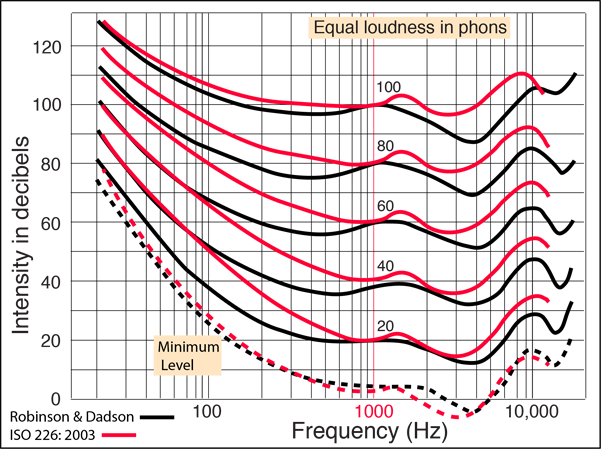
\includegraphics[width=0.7\linewidth]{Chapter_2/figures/equal_loudness_curve.png}
  \caption{Equal-loudness contours comparing the Robinson and Dadson determinations in 1956 (black lines) with the revised ISO~226:2003 standard (red lines). Each contour connects frequency--SPL pairs perceived as equally loud. The label on each contour indicates its loudness level in phons, which corresponds to the SPL of an equally loud 1\,kHz pure tone. The dashed lines represent the minimum threshold of hearing \cite{robinson1956equal_loudness,iso2262003,equal_loudness}.}
  \label{fig:bg_equal_loudness}
\end{figure}

In loudness-related analysis, the \emph{phon} is still not the most convenient end point because it does not provide a linear scale of subjective loudness. A sound of 80 phons is not perceived as twice as loud as one of 40 phons. A more useful perceptual unit is the \emph{sone}, which is designed such that its value is linearly proportional to perceived loudness. A sound of 2 sones is perceived as twice as loud as a 1-sone sound. In practice, there are two common routes to obtain sone values.

\begin{table}[!htbp]
\centering
\caption{Approximate correspondence between phons and sones.}
\label{tab:phons_sones_simple}
\setlength{\tabcolsep}{10pt}
\fontsize{11pt}{13pt}\selectfont
\renewcommand{\arraystretch}{1.3}
\begin{tabular}{lccccccccc}
\toprule
\textbf{Phons} & 40 & 50 & 60 & 70 & 80 & 90 & 100 & 110 & 120\\
\textbf{Sones} & 1  & 2  & 4  & 8  & 16 & 32 & 64  & 128 & 256\\
\bottomrule
\end{tabular}
\end{table}

The first is to convert the loudness level in phons into sones. Based on the loudness relations summarised by Backus~\cite{backus1977acoustical}, Table~\ref{tab:phons_sones_simple} gives the anchor pairs, while intermediate values are obtained by the standard approximation (where the unit of $L_N$ is phons):
\begin{equation}
S =
\begin{cases}
2^{(L_N-40)/10}, & L_N \ge 40,\\[4pt]
(L_N/40)^{2.642}, & L_N < 40.
\end{cases}
\label{eq:bg:phon_to_sone}
\end{equation}
The second route is to approximate perceived loudness directly from physical intensity via Stevens' power law, bypassing the need to read $L_N$ from equal-loudness contours:
\begin{equation}
S = \frac{1}{15.849}\left(\frac{I}{I_0}\right)^{0.3},
\label{eq:bg:stevens_power}
\end{equation}
where $S$ denotes loudness in sones \cite{backus1977acoustical}. In MIR practice, the first route is usually preferable because frequency dependence has already been made explicit through equal-loudness contours and can later be refined further by critical-band modelling.

\subsection{Bark-scale and critical bands}

The pure-tone framework above explains how physical level relates to perceived loudness for isolated tones. For musical audio, however, it is not sufficient to treat each FFT bin as an independent loudness event. Singing, piano, and polyphonic textures distribute energy across harmonics, formants, accompaniment, and transients, and the auditory system integrates nearby components within auditory filters whose bandwidth varies with frequency. This is the psychoacoustic motivation for \emph{critical bands} \cite{zwicker1999psychoacoustics}.

The audible frequency range is conventionally organised into 24 critical bands indexed by the Bark scale, a psychoacoustic concept originally proposed by Zwicker in 1960 \cite{zwicker1960unterteilung}. Table~\ref{tab:bark_table} shows the approximate relation between Bark index, frequency, and bandwidth. The important point is that Bark is a perceptual frequency coordinate rather than a loudness value: low-frequency bands are relatively narrow in Hz, whereas higher-frequency bands become progressively broader. For sampled audio, the usable part of this scale is bounded by the Nyquist frequency. The table therefore provides the practical basis for deciding which Bark bands are retained at a given sampling rate, with the highest band treated according to the implementation when its frequency range is only partially available. 

\begin{table*}[!htbp]
    \centering
    \caption{Approximate relation between critical-band rate in Bark and frequency in Hz. The full psychoacoustic scale spans 24 critical bands.}
    \label{tab:bark_table}
    \setlength{\tabcolsep}{4.6pt}
    \fontsize{11pt}{13pt}\selectfont
    \renewcommand{\arraystretch}{1.18}
    \begin{tabular}{ccc@{\hspace{8pt}}ccc@{\hspace{8pt}}ccc}
        \toprule
        \makecell[c]{\textbf{Critical}\\[1pt]\textbf{band rate}\\[1pt]\textbf{$z$ [Bark]}} &
        \makecell[c]{\textbf{Frequency}\\[1pt]\textbf{$f$ [Hz]}} &
        \makecell[c]{\textbf{$\Delta f$}\\[1pt]\textbf{[Hz]}} &
        \makecell[c]{\textbf{Critical}\\[1pt]\textbf{band rate}\\[1pt]\textbf{$z$ [Bark]}} &
        \makecell[c]{\textbf{Frequency}\\[1pt]\textbf{$f$ [Hz]}} &
        \makecell[c]{\textbf{$\Delta f$}\\[1pt]\textbf{[Hz]}} &
        \makecell[c]{\textbf{Critical}\\[1pt]\textbf{band rate}\\[1pt]\textbf{$z$ [Bark]}} &
        \makecell[c]{\textbf{Frequency}\\[1pt]\textbf{$f$ [Hz]}} &
        \makecell[c]{\textbf{$\Delta f$}\\[1pt]\textbf{[Hz]}} \\
        \midrule
        0 & 0    & 100 & 9  & 1080  & 190 & 18 & 4400  & 900  \\
        1 & 100  & 100 & 10 & 1270  & 210 & 19 & 5300  & 1100 \\
        2 & 200  & 100 & 11 & 1480  & 240 & 20 & 6400  & 1300 \\
        3 & 300  & 100 & 12 & 1720  & 280 & 21 & 7700  & 1800 \\
        4 & 400  & 110 & 13 & 2000  & 320 & 22 & 9500  & 2500 \\
        5 & 510  & 120 & 14 & 2320  & 380 & 23 & 12000 & 3500 \\
        6 & 630  & 140 & 15 & 2700  & 450 & 24 & 15500 & --   \\
        7 & 770  & 150 & 16 & 3150  & 550 &    &       &      \\
        8 & 920  & 160 & 17 & 3700  & 700 &    &       &      \\
        \bottomrule
    \end{tabular}
\end{table*}
A common analytic approximation from physical frequency $f$ in kHz to Bark rate $z$ is
\begin{equation}
z(f_{\mathrm{kHz}}) = 13\arctan(0.76 f_{\mathrm{kHz}}) + 3.5\arctan\!\left(\frac{f_{\mathrm{kHz}}^2}{7.5^2}\right),
\label{eq:bg:bark_mapping}
\end{equation}
where $f_{\mathrm{kHz}}$ denotes frequency in kHz \cite{pampalk2002content,pampalk2004exploring,zwicker1999psychoacoustics}. This equation defines the Bark coordinate itself. It does not yet compute loudness. 

Once this mapping is available, a linear-frequency spectrogram can be regrouped into Bark bands. If $P(k,t)$ denotes the power at frequency bin $k$ and frame $t$, and $\mathcal{B}_b$ is the set of bins whose centre frequencies fall into Bark band $b$, then the Bark spectrogram for the retained Bark bands is
\begin{equation}
B(b,t) = \sum_{k \in \mathcal{B}_b} P(k,t),
\qquad
\mathcal{B}_b = \{k \mid z_{b-1} \le z(f_k) < z_b\}.
\label{eq:bg:bark_spectrogram}
\end{equation}
This step changes the spectral coordinate system from Hz to critical-band rate. The actual loudness model is introduced in the next subsection, where auditory weighting, spectral spreading, and nonlinear conversion are applied to obtain specific loudness.


\subsection{Bark-scale specific loudness and total loudness}
Among psychoacoustic-informed audio representations, Bark-scale specific loudness (BSSL) is designed to represent how perceived loudness is distributed across auditory critical bands, as human perception of loudness is more sensitive to certain frequency bands \cite{zwicker1999psychoacoustics,zwicker2007psychoacoustics}. Because it preserves both spectral location and perceptual magnitude, BSSL is well suited to dynamics-related MIR tasks \cite{narang2024automatic,he2026dynest}. While several BSSL extraction methods exist, such as DIN 45631/A1: 2010 \cite{din45631a1_2010} and ISO 532-1:2017 \cite{iso532_1_2017}, they are designed for industrial noise and sound quality assessment, assuming specific sound profiles. In MIR, however, music signals are typically highly polyphonic with negligible background noise. Therefore, the implementation proposed by Pampalk et al. \cite{pampalk2002content, pampalk2004exploring} is widely adopted. The extraction pipeline is defined as follows.

First, the audio is converted to mono, peak-normalised to $-1\,\mathrm{dBFS}$, and resampled to a chosen sampling rate $f_s$ that preserves the spectral range required by the downstream MIR task. A short-time Fourier transform (STFT) then yields the complex spectrogram $X(k,t)$, where $t$ denotes the frame index and $k$ the frequency-bin index. The power spectrogram $P(k,t)$ is then formed using window-energy normalisation:
\begin{equation}
P(k,t)=\frac{|X(k,t)|^2}{(\sum_{n=0}^{N-1} w[n])^2}.
\end{equation}
To approximate the frequency response of the human outer and middle ear, Terhardt's weighting function $W_{\mathrm{dB}}(f_k)$ \cite{terhardt1979outerear} is applied. This weighting is specified in decibels, where $f_k$ denotes the centre frequency (in $\mathrm{kHz}$) of the $k$-th bin:
\begin{equation}
W_{\mathrm{dB}}(f_k) = -3.64\,f_k^{-0.8} + 6.5\,e^{-0.6\,(f_k-3.3)^2} - 10^{-3}\,f_k^{4}.
\end{equation}
Since $P(k,t)$ is a linear-scale power quantity, this weighting must be converted to a linear power gain before being applied:
\begin{equation}
W(f_k)=10^{\,W_{\mathrm{dB}}(f_k)/10},
\qquad
P_W(k,t)=P(k,t) \cdot W(f_k).
\end{equation}
The weighted power spectrogram $P_W(k,t)$ is then mapped to the Bark scale by the same pooling operation defined in Equation~\eqref{eq:bg:bark_spectrogram}, yielding the weighted Bark spectrogram $B_W(b,t)$. In sampled audio, the number of usable Bark-band channels is constrained by the Nyquist frequency. Let $B_{\mathrm{ret}}$ denote the number of Bark channels retained after applying this sampling-rate and implementation constraint; the retained bands are therefore $b \in \{1,\ldots,B_{\mathrm{ret}}\}$. The notation below uses $B_{\mathrm{ret}}$ rather than fixing BSSL to a nominal 22- or 24-band representation.

Taking into account spectral masking over neighbouring Bark bands, where a strong component can make weaker nearby components harder to perceive, the spreading function proposed by Schroeder et al.~\cite{schroeder1979masking} is applied:
\begin{equation}
G_{\mathrm{dB}}(\Delta)
=15.81 + 7.5(\Delta +0.474)
-17.5\sqrt{1+(\Delta +0.474)^2},
\label{eq:bg:spreading_function_db}
\end{equation}
where $\Delta=b-j$ denotes the distance from source band $j$ to target band $b$. Since $G_{\mathrm{dB}}$ is specified in decibels and $B_W(b,t)$ is represented on a linear power scale, the spreading function is converted to a linear power gain:
\begin{equation}
G(\Delta)=10^{G_{\mathrm{dB}}(\Delta)/10}.
\label{eq:bg:spreading_function_linear}
\end{equation}
The spread Bark-scale excitation is then computed as
\begin{equation}
\widetilde{B}_W(b,t)
=
\sum_{j=1}^{B_{\mathrm{ret}}} B_W(j,t)\,G(b-j),
\qquad b=1,\ldots,B_{\mathrm{ret}}.
\label{eq:bg:spread_bark_excitation}
\end{equation}
This step reflects a fundamental psychoacoustic principle: loudness perception is not a naive sum of independent narrowband energies, but involves auditory interaction across neighbouring critical bands.

Traditionally, converting a sound representation expressed in sound-pressure level to the perceptual \emph{phon} scale requires mapping through equal-loudness contours. For the spread Bark excitation $\widetilde{B}_W(b,t)$, however, the previously applied outer/middle-ear weighting, Bark-band pooling, and spectral spreading have already introduced frequency-dependent auditory adjustments. Therefore, this implementation does not apply an additional equal-loudness contour lookup at this stage. Instead, the logarithmic level of $\widetilde{B}_W(b,t)$ is treated as a phon-like loudness-level input for the subsequent sone conversion. Following Zwicker's 1999 pipeline \cite{zwicker1999psychoacoustics,pampalk2002content,pampalk2004exploring}, this logarithmic conversion is defined as:
\begin{equation}
L_B(b,t)=\max\!\left(0,\,10\log_{10}\!\left(\widetilde{B}_W(b,t)+\epsilon\right)\right),
\label{eq:bg:spread_bark_level}
\end{equation}
where $\epsilon$ is a small constant used to avoid taking the logarithm of zero. The level $L_B(b,t)$ then serves as the input for the phon-to-sone conversion in Equation~\eqref{eq:bg:phon_to_sone}. The resulting Bark-scale specific loudness (BSSL), denoted as $N'(b,t)$, represents the specific loudness for Bark band $b$ at frame $t$:
\begin{equation}
N'(b,t)=
\begin{cases}
2^{(L_B(b,t)-40)/10}, & L_B(b,t)\ge40,\\[4pt]
(L_B(b,t)/40)^{2.642}, & L_B(b,t)<40.
\end{cases}
\label{eq:bg:bssl}
\end{equation}
The resulting BSSL is a $B_{\mathrm{ret}}$-dimensional time--frequency representation of perceived loudness, with $N'(b,t)$ measured in sone/Bark. The corresponding Bark-scale total loudness (BSTL), denoted as $N_{\mathrm{tot}}(t)$, collapses this frequency-resolved representation into a single time-varying scalar by integrating over the retained Bark axis:
\begin{equation}
N_{\mathrm{tot}}(t)=\int_{0}^{B_{\mathrm{ret}}} N'(z,t)\,dz.
\label{eq:bg:total_loudness_cont}
\end{equation}
In the discrete retained-band implementation, this is approximated as:
\begin{equation}
N_{\mathrm{tot}}(t)\approx \sum_{b=1}^{B_{\mathrm{ret}}} N'(b,t)\Delta z,
\qquad \Delta z = 1.
\label{eq:bg:total_loudness_discrete}
\end{equation}
In other words, BSSL preserves where loudness is located in the auditory spectrum, whereas BSTL retains only the overall perceptual magnitude at each time frame. The two representations are therefore complementary: BSTL is appropriate when a compact loudness curve is sufficient, while BSSL is preferable when the spectral distribution of loudness is expected to carry musically relevant information. This distinction is visualised later in Figure~\ref{fig:bg_temporal_units}(b)--(c), where BSSL retains the Bark-wise loudness distribution while BSTL reduces it to a single trajectory.

\subsection{Other Audio Representations Related to Loudness}

Besides explicit loudness measures, MIR also relies on time--frequency representations that retain amplitude information with different degrees of perceptual relevance. At the simplest level, short-time RMS energy provides a frame-level estimate of signal power and is widely used as a baseline descriptor of local intensity. However, RMS remains only a coarse proxy for perceived loudness: it reduces each analysis frame to a single scalar and therefore cannot represent how dynamic impression also depends on the spectral distribution of energy, rather than on overall level alone. This limitation is important because perceived dynamics are not determined by level alone. The pitch, loudness, and timbre can jointly affect perceived instrument dynamics, and broader MIR work on musical affect and tension also treats loudness as only one cue among several acoustic factors \cite{panda2023audiofeatures,fabiani2011influence,barchet2024tensemusic}.

For this reason, sub-band spectral representations are often more informative than scalar energy features for dynamics-related MIR tasks, especially the Mel-based representations \cite{fu2011survey,nam2019deeplearningaudio,panda2023audiofeatures,mcloughlin2026spectrogramfeatures}. A Mel spectrogram aggregates spectral energy into perceptually motivated frequency bands, preserving not only how much energy is present but also where that energy lies in the spectrum \cite{slaney1998auditory}. A log-Mel spectrogram further applies logarithmic compression, reducing the dominance of very large amplitudes, stabilising the representation across a wide dynamic range, and making it more consistent with the nonlinear character of loudness perception. Nevertheless, log-Mel does not explicitly model human loudness perception. Consequently, recent works in loudness estimation typically employ log-Mel as a standard baseline against which the superior loudness modelling capabilities of BSSL are compared \cite{narang2024automatic, he2026dynest}.

Compact cepstral features such as MFCCs and BFCCs provide lower-dimensional summaries of filterbank energies on perceptual frequency scales. MFCCs are derived from Mel-scale filterbank energies and have long been used in speech and music modelling \cite{davis1980comparison,logan2000mel}, while BFCCs apply the same general cepstral idea on the Bark scale \cite{herrera2010bfcc}. These features are attractive when compactness, decorrelation, and robust timbral description are important, and they remain common in MIR applications such as music classification and instrument recognition \cite{fu2011survey,panda2023audiofeatures,chen2024interpreting}. However, this compression is also their main limitation for fine-grained dynamics analysis: by transforming sub-band energies into a compact cepstral representation, they remove part of the band-wise structure that may carry local loudness, resonance, and spectral-balance cues. BFCCs inherit the same trade-off on the Bark scale. For dynamics-focused modelling, directly retaining Mel/Bark band energies or using specific-loudness representations is therefore usually easier to justify than relying on cepstral summaries alone \cite{mcloughlin2026spectrogramfeatures,narang2024automatic,he2026dynest,kondo2025perceivedvibrato}.

By contrast, the Constant-Q Transform (CQT) is designed around logarithmically spaced frequency bins whose spacing aligns closely with musical pitch \cite{brown1991constantq}. This makes CQT well suited to pitch-, harmony-, and transcription-oriented tasks, where the representation benefits from a frequency axis organised according to musical scale structure \cite{cheuk2020impact,mcloughlin2026spectrogramfeatures}. CQT can still retain amplitude variation implicitly, but its frequency organisation is not based on critical-band loudness or specific-loudness modelling. For that reason, CQT is better understood as a pitch- and harmony-oriented representation than as a primary representation for loudness or musical dynamics. 


\section{Dynamics in MIDI and Score}
\label{sec:bg:dynamics_midi_score}

Audio captures the sounding result of dynamics: pressure variation, spectral energy, and perceived loudness. Symbolic formats describe dynamics through a different kind of abstraction. In a score, dynamics are written as \emph{dynamic markings}: sparse, human-readable instructions such as \textit{p}, \textit{f}, and \textit{crescendo}. In MIDI, dynamics are represented primarily by \emph{velocity}: a dense, machine-readable control value attached to individual note onsets. These two representations are connected through performance, but they are not interchangeable measurements. Dynamic markings describe an expressive intention over musical context; MIDI velocity records or controls local note attack. The gap between them is therefore a central modelling problem rather than a formatting problem.


\subsection{Dynamic markings as macro-level musical instructions}
\label{sec:bg:dynamic_markings}

Dynamic markings are the conventional score vocabulary for notated loudness and dynamic change. They include static markings such as \textit{pp}, \textit{p}, \textit{mp}, \textit{mf}, \textit{f}, and \textit{ff}, as well as directional indications such as \textit{crescendo}, \textit{diminuendo}, and hairpins. Although a marking is printed at a specific visual position, its musical scope is usually broader than that position. A single \textit{p} may govern a phrase, a texture, or a formal region until a later marking or musical event changes the dynamic state. A crescendo indicates a tendency over a span, not an isolated value at one note.

The crucial point is that dynamic markings are not calibrated volume labels. They are relational instructions. A \textit{forte} passage is not defined by a fixed sound-pressure level, nor does a \textit{piano} passage prescribe a fixed physical intensity. The intended realisation depends on register, texture, melodic role, harmonic tension, instrumentation, acoustic setting, historical style, and the performer's interpretive priorities. A melody marked \textit{p} may require more acoustic energy than an accompaniment marked \textit{mf}; an inner voice may remain physically soft while sounding perceptually salient because of register or timbral contrast. This context dependence is central to empirical work on the relation between dynamic markings and performed loudness \cite{kosta2014dynpiano,kosta2016mapping}.

Dynamic markings are therefore macro-level representations. They compress many local performance decisions into a small number of expressive symbols. Their value lies precisely in this compression: they allow a composer or editor to specify the character of a passage without prescribing every note attack. Expressive performance research treats dynamics as one dimension of a broader transformation from score structure into timing, intensity, articulation, and timbral choices \cite{cancinoChacon2018computational,grachten2012linear}. Recent modelling work on piano performance also shows that performers produce systematic dynamic profiles from phrase structure, metrical position, register, and style, even when explicit dynamic markings are removed \cite{jones2023probingdyn}. Dynamic markings should therefore be understood as musically precise but physically under-specified instructions.

For MIR, this has a direct consequence. A dynamic marking is a weak but meaningful label. It is weak because it does not determine exact amplitude, MIDI velocity, or loudness. It is meaningful because it identifies the expressive region that a listener, performer, or teacher can recognise in the score. In this thesis, the term \emph{dynamic markings} is used for this score-facing representation throughout, and its practical coordinate is the beat, bar, or phrase rather than the audio frame.

\subsection{MIDI velocity as micro-level performance control}
\label{sec:bg:midi_velocity}

MIDI velocity is a different kind of representation. It is attached to a note onset rather than to a phrase or region. In conventional MIDI performance data, a sounding note onset carries a discrete velocity value on a finite integer scale. In a chord, each note may have a different velocity. In a rapid passage, every note can carry its own local attack value. MIDI velocity is therefore a micro-level representation: it serialises note-level actions rather than summarising the expressive state of a passage.

The word \emph{velocity} is often described informally as key-strike force. For keyboard instruments this is useful but imprecise. In sensor-equipped acoustic pianos, the recorded value is more accurately treated as a discretised proxy for key or hammer motion near the note attack. Studies of computer-controlled pianos distinguish the player's physical action, the hammer--string interaction, the measured control value, and the resulting acoustic signal \cite{goebl2003role,goebl2004piano}. Large piano datasets such as MAESTRO use this property to provide aligned audio and MIDI data with key-strike velocity labels, making note-level velocity a practical target for MIR systems \cite{hawthorne2019maestro}.

MIDI velocity is exact as symbolic data. A note with velocity 80 remains velocity 80 when the MIDI file is copied, edited, or passed to a model. It is also mechanical in the sense that it refers to a local performance control: how strongly a note attack is executed or how strongly a synthesiser should respond. This objectivity is one reason why velocity is attractive for automatic transcription, expressive rendering, and symbolic performance modelling \cite{ewert2011est,kim2023score,kim2024method}.

However, exactness in the data structure does not imply universality in sound. MIDI velocity is not loudness, not amplitude, and not a dynamic marking. It is a control parameter whose acoustic effect depends on the instrument, renderer, register, sample layer, synthesis design, and recording chain. Dannenberg's analysis of MIDI velocity shows that different synthesisers and patches implement substantially different velocity-response curves \cite{dan2006psy}. Thus, a MIDI value can be objective without being perceptually absolute. It is exact as a note-level control value, but relative as an acoustic and musical quantity.

\subsection{Bridging the gap between dynamics representations}
\label{sec:bg:dynamics_bridge}

A tempting solution is to convert between MIDI velocity and dynamic markings with a fixed lookup table. Such a table might assign low velocities to \textit{p}, middle velocities to \textit{mf}, and high velocities to \textit{f}; the inverse table would assign each printed marking a nominal playback velocity. Table~\ref{tab:dyn_midi_main} illustrates how representative notation software (Logic Pro, MuseScore, Sibelius, Finale, Dorico) implements such mappings between score-dynamics symbols, loudness-related scales, and MIDI velocity values. This is useful for deterministic playback in notation software and digital audio workstations. It is not a reliable model of musical dynamics. Formally, the naive assumption is that a single scalar function can map a note-level value $v$ to a score-level marking $d$:
\begin{equation}
d = g(v), \qquad
d \in \{\textit{pp}, \textit{p}, \textit{mp}, \textit{mf}, \textit{f}, \textit{ff}\}.
\label{eq:bg_velocity_to_dynamic_naive}
\end{equation}

\begin{table*}[!htbp]
\centering
\scriptsize
\caption[Score-dynamics vocabulary, loudness-related scales, and MIDI velocity scales]{Illustrative correspondences between score-dynamics vocabulary, loudness-related scales, and MIDI velocity values in representative music software.}
\label{tab:dyn_midi_main}
\setlength{\tabcolsep}{2pt}
\fontsize{10pt}{11pt}\selectfont
\renewcommand{\arraystretch}{1.2}
\begin{tabular}{clccccc}
\toprule
\multicolumn{1}{c}{\textbf{Loudness}} &
\multicolumn{1}{c}{\textbf{Score Dynamics}} &
\multicolumn{5}{c}{\textbf{MIDI Velocity}} \\
\cmidrule(lr){1-1} \cmidrule(lr){2-2} \cmidrule(l){3-7}
\makecell[c]{\textbf{sones}} &
\makecell[c]{\textbf{Symbol \& Meaning}} &
\makecell{\textbf{Logic Pro} \cite{logicpro-stepinput}} &
\makecell{\textbf{MuseScore} \cite{musescore-dynamic-source}} &
\makecell{\textbf{Sibelius} \cite{sibelius7sounds}} &
\makecell{\textbf{Finale} \cite{palamara2020dynamic}} &
\makecell{\textbf{Dorico} \cite{palamara2020dynamic}} \\
\midrule
128 & \textit{ffff}: threshold of pain    & --  & 127 & --  & 127 & 123 \\
64  & \textit{fff}: yelling               & 127 & 126 & 127 & 114 & 119 \\
32  & \textit{ff}: very loud              & 112 & 112 & 113 & 101 & 101 \\
16  & \textit{f}: loud                    & 96  & 96  & 98  & 88  & 89  \\
8   & \textit{mf}: normal speaking        & 80  & 80  & 84  & 75  & 77  \\
8   & \textit{mp}: normal speaking        & 64  & 64  & 71  & 62  & 61  \\
4   & \textit{p}: soft                    & 48  & 49  & 61  & 49  & 46  \\
2   & \textit{pp}: almost a whisper       & 32  & 33  & 39  & 36  & 25  \\
1   & \textit{ppp}: whispering            & 16  & 16  & 20  & 23  & 14  \\
0   & \textit{pppp}: threshold of hearing & --  & 10  & --  & 10  & 5   \\
\bottomrule
\end{tabular}
\\[0.5ex]
\parbox{0.98\textwidth}{\footnotesize
\textit{Notes.}
The table is illustrative rather than normative. The listed values reflect representative software mappings and do not define a universal conversion between score dynamics and performed loudness. Logic Pro entries refer to Apple's documented step-input velocity buttons rather than score-playback dynamics~\cite{logicpro-dynamics-visual,logicpro-stepinput}. Finale and Dorico entries follow the comparative values reported in~\cite{palamara2020dynamic}.
}
\end{table*}

The failure of this assumption has two main causes. Both follow from the same representational problem: MIDI velocity, perceived loudness, and score dynamics live on different coordinates. A velocity value is attached to a note onset, a loudness impression is distributed over time and frequency, and a score marking describes a contextual musical state. Any direct lookup table therefore discards the intermediate stages that make dynamics musically meaningful.

\paragraph{Instrument dependence.}
MIDI velocity is physically arbitrary across instruments. The same velocity value may trigger different amplitudes, spectra, sample layers, envelopes, or synthesis behaviours depending on the instrument. Velocity 80 on a sampled grand piano may produce a bright attack and strong hammer noise; velocity 80 on a soft synthesiser patch may mainly open a filter or change an envelope; velocity 80 on another renderer may produce only a small loudness change. Even within piano, the relationship between velocity and acoustic output depends on pitch, register, hammer mechanics, resonance, microphone placement, and the reproduction system \cite{goebl2003role,dan2006psy}. A fixed velocity threshold therefore cannot define an instrument-independent boundary between \textit{mp}, \textit{mf}, and \textit{f}.

This problem also affects the reverse direction. Assigning \textit{f} to a single nominal velocity may be adequate for rough playback, but it ignores the instrument-specific response needed to make a passage sound forte-like. A convincing \textit{forte} on one instrument may require a different velocity range, spectral balance, or articulation strategy on another. Rule-based approaches to musical dynamics can impose useful rendering conventions, but they cannot remove the instrument dependence of the underlying control-to-sound mapping \cite{berndt2010modelling}.

\paragraph{Perceptual loudness and performer style.}
The second obstacle is perceptual and musical. Human listeners do not hear MIDI velocity values. They hear loudness, salience, balance, and expressive shape. Loudness perception is nonlinear and depends on frequency-dependent sensitivity, critical-band interaction, masking, and temporal integration \cite{zwicker1999psychoacoustics,zwicker2007psychoacoustics}. A dense chord played with moderate note velocities can be perceived as louder than a single note with a higher velocity because total loudness depends on how energy is distributed across frequency bands and time. Conversely, a high-velocity note may be masked by surrounding texture or may fail to dominate if it occupies a less perceptually prominent register.

Performer style adds another layer. A pianist's realisation of \textit{forte} is shaped by phrase direction, metrical hierarchy, historical idiom, local texture, and personal expressive strategy. Empirical studies of dynamic markings and performed loudness show that the mapping between notated symbols and realised loudness is learnable within constrained contexts but unstable across pieces, performances, and performers \cite{kosta2016mapping}. Related modelling work shows that different pianists can agree on broad dynamic tendencies while still differing in the local strategies used to produce them \cite{jones2023probingdyn}. A dynamic marking is therefore not a target number; it is an interpretive category.

The bridge between MIDI velocity and dynamic markings must consequently model context. It must account for the instrument that turns velocity into sound, the auditory system that turns sound into perceived loudness, and the performer or annotator who turns musical context into an expressive label. A lookup table collapses these stages into one scalar threshold. The later chapters of this thesis instead treat symbolic dynamics recovery as a structured MIR problem: note-level velocity estimation, score-informed correction, and beat-synchronous dynamic-marking recovery address different parts of the same many-to-many relationship between machine-readable performance control and human-readable musical notation.

\section{Expressive MIR: Historical Overview and Task Landscape}
\label{sec:bg:expressive_mir}

The previous three sections defined what \emph{dynamics} means at each layer of representation. They did not yet describe how the MIR community has tried to recover those representations from data. The present section serves that purpose. It is the first literature-review section of the chapter, and it sets up the three task-specific reviews that follow (Sections~\ref{sec:bg:velocity}, \ref{sec:bg:scoredyn}, and~\ref{sec:bg:synthesis}).

\subsection{Performance research as a precursor to expressive MIR}

Music performance research is the historical reason why dynamics cannot be treated as a small extension to note transcription. Earlier studies of expressive performance showed that timing and dynamics are shaped by phrase structure, metre, accent, local tension, and instrumental constraints \cite{goebl2003role,cancinoChacon2018computational}. These findings matter for MIR because they make dynamics different from pitch or onset. A pitch label can often be judged against a relatively stable musical event, whereas a dynamics label depends on how a performer interprets that event in context.

This does not mean that expressive MIR should abandon discrete labels. It means that the label must be tied to the right musical coordinate. A note-level velocity is meaningful when the task is to control the rendering of individual note events. A score-level dynamic marking is meaningful when the task is to annotate a metrical or phrase-level change in loudness. A frame-level loudness contour is useful as acoustic evidence, but it is not itself a score annotation. Performance research therefore supplies more than motivation: it explains why representation choice is a validity condition. A system can be accurate with respect to one dynamics representation while being musically inappropriate for another.

\subsection{From note transcription to expressive transcription}

Classical AMT focused on recovering pitch content and note boundaries. Recent deep-learning systems have made this problem increasingly reliable for piano, especially on datasets such as MAESTRO and MAPS \cite{amt2019ov,hawthorne2018onsets,hawthorne2021trans,kong2021hpt,toyama2023hft,yan2021semicrf,yan2024semicrf}. Table~\ref{tab:amt_sota} should therefore be read not only as a benchmark summary, but as evidence of a shift in the bottleneck. For piano, note and note-plus-offset scores are now strong enough that the remaining expressive layer becomes visible: velocity-aware performance remains weaker, and the gap is not simply a matter of detecting more notes. It reflects the difficulty of estimating how strongly each known note should be rendered.

The multi-instrument case exposes a second bottleneck. On MusicNet and related corpora, the transcription problem is harder, and velocity-aware evaluation is often absent because reliable note-level velocity supervision is not available outside sensor-equipped piano datasets. This creates an asymmetry that runs through the thesis: piano provides the cleanest supervised setting for velocity recovery, while other instruments often provide audio and aligned notes but no trustworthy velocity labels. Expressive transcription is therefore not a detached field from AMT. It is the next layer of symbolic recovery once note content and timing are sufficiently constrained, and it requires different assumptions about supervision and evaluation.

\begin{table*}[!h]
\centering
\caption{Representative AMT results across MAPS, MAESTRO, and MusicNet. The numbers show that velocity-aware transcription remains substantially harder than note transcription.}
\label{tab:amt_sota}
\setlength{\tabcolsep}{3.7pt}
\fontsize{10pt}{11pt}\selectfont
\renewcommand{\arraystretch}{1.2}

\begin{tabular}{
>{\centering\arraybackslash}m{3.0cm}
>{\centering\arraybackslash}m{1.0cm}
>{\centering\arraybackslash}m{3.5cm}
>{\centering\arraybackslash}m{1.2cm}
>{\centering\arraybackslash}m{1.1cm}
>{\centering\arraybackslash}m{1.5cm}
>{\centering\arraybackslash}m{2.2cm}
}
\toprule
\textbf{Method} & \textbf{Year} & \textbf{Model} & \makecell{\textbf{F1} \\ \textbf{frame}} & \makecell{\textbf{F1} \\ \textbf{note}} & \makecell{\textbf{F1} \\ \textbf{note\&off}} & \makecell{\textbf{F1} \\ \textbf{note\&off\&velo}} \\
\midrule

\multicolumn{7}{c}{\textbf{MAPS (piano)}} \\
\midrule
OaF \cite{hawthorne2018onsets} & 2018 & CRNN & 78.30 & 82.29 & 50.22 & 35.39 \\
Wu et al. \cite{wu2019semantic} & 2019 & CNN & 86.73 & -- & -- & -- \\
ADSR \cite{kelz2019adsr} & 2019 & CNN + HMM & 77.16 & 81.38 & 56.08 & -- \\
hFT-Trans \cite{toyama2023hft} & 2023 & Transformer & 82.89 & 85.14 & 66.34 & 48.20 \\
\midrule

\multicolumn{7}{c}{\textbf{MAESTRO (piano)}} \\
\midrule
OaF$^\dagger$ \cite{hawthorne2018onsets} & 2018 & CRNN & 87.82 & 94.93 & 79.65 & 76.05 \\
HPT$^\dagger$ \cite{kong2021hpt} & 2021 & CRNN & 90.15 & 96.77 & 84.45 & 83.02 \\
SemiCRFs$^\dagger$ \cite{yan2021semicrf} & 2021 & CRNN + SemiCRF & 91.11 & 96.51 & 88.72 & 87.75 \\
Seq2Seq \cite{hawthorne2021trans} & 2021 & Transformer & -- & 96.01 & 83.94 & 82.75 \\
HPT-T \cite{kong2021hpt} & 2021 & CRNN & 90.09 & 96.77 & 83.20 & 81.90 \\
HPPNet-sp \cite{wei2022hppnet} & 2022 & CRNN & 93.15 & 97.18 & 83.80 & 82.24 \\
hFT-Trans \cite{toyama2023hft} & 2023 & Transformer & 93.24 & 97.44 & 90.53 & 89.48 \\
Transkun v2 \cite{yan2024semicrf} & 2024 & Trans. + SemiCRF & 95.35 & 98.32 & 93.48 & 92.94 \\
\midrule

\multicolumn{7}{c}{\textbf{MusicNet (multi-instrument)}} \\
\midrule
Wu et al. \cite{wu2019semantic} & 2019 & CNN & 73.70 & -- & -- & -- \\
ReconVAT \cite{cheuk2021reconvat,gardner2022mt3} & 2021 & U-Net & 48.0 & 29.0 & 11.0 & -- \\
MT3 \cite{gardner2022mt3} & 2022 & Transformer & 68.0 & 50.0 & 33.0 & -- \\
PerceiverTF \cite{lu2023perceivertf} & 2023 & Trans. + Perceiver & 63.7 & 46.1 & 29.0 & -- \\
PF2N$^\S$ \cite{kim2025pf2n} & 2025 & PF2N + Perceiver & 64.5 & 47.5 & 30.7 & -- \\
\bottomrule
\end{tabular}
\vspace{0.5ex}
\parbox{0.98\linewidth}{\footnotesize
$^\dagger$ Re-evaluation on MAESTRO v3 by SemiCRF paper. \\
}
\end{table*}

Expressive AMT is therefore not a separate field detached from AMT. It is the next layer of symbolic recovery once note content and timing become reasonably stable. The thesis positions its contributions as extensions of AMT towards expressive and editable symbolic outputs rather than as alternatives to note transcription.

\subsection{Three task lines of dynamics-related MIR}
The literature separates most clearly not by model family, but by what musical structure is assumed to be trustworthy. This is the organising principle used in the rest of the chapter.

\paragraph{Note-level MIDI velocity recovery.}
The first task line assumes that the note events are already known and asks only for the missing per-note velocity values. This setting is attractive because it preserves the composition exactly: pitch, onset, and duration remain fixed, while the model restores an editable control layer. Its limitation is equally clear. MIDI velocity is a renderer-facing parameter, not a direct measurement of perceived loudness or score dynamics. It is therefore well suited for expressive rendering and MIDI data curation, but it should not be treated as a universal representation of musical dynamics.

\paragraph{Beat-synchronous score-dynamics recovery.}
The second task line aims at dynamic markings such as \emph{p}, \emph{mf}, and \emph{f}. Here the output is not a velocity value attached to every note, but a sparse symbolic description aligned with the metrical structure of the score. This changes both the temporal unit and the semantics of the target. A score marking is intentionally coarse and contextual; it describes a region of musical interpretation rather than the intensity of a single event. Methods in this line must therefore model loudness evidence together with beats, downbeats, and change points, rather than treating dynamics as frame-wise audio classification alone.

\paragraph{Renderer-based and proxy-based recovery.}
The third task line appears when the target-domain velocity label is missing. In this case, supervised learning from ground-truth velocities is not available, even if audio and aligned notes exist. A renderer or differentiable proxy can then provide an indirect training signal: predicted velocities are judged by whether their rendered dynamics match the performance audio. This formulation is weaker than direct supervision, but it is not merely a workaround. It changes the claim being made. The recovered value is a usable dynamics coordinate for rendering or analysis under a specified synthesis condition, rather than a canonical physical measurement of the performer's gesture.

\subsection{Cross-cutting validity: temporal units, alignment, and priors}
\label{sec:bg:expressive_mir:validity}

Independently of the specific task line, three cross-cutting concerns determine whether a dynamics-related MIR system is even well-posed: which temporal unit indexes the prediction, whether the supervision is aligned, and what structural prior makes an underdetermined target tractable.

\paragraph{Temporal units.}
A dynamics-related event can be represented at several temporal resolutions, and each resolution carries a different modelling assumption. At the densest level, log-Mel and BSSL provide frame-level time--frequency evidence, while BSTL collapses the Bark-wise loudness distribution into a frame-level loudness trajectory. At the symbolic level, note onsets and note events index the local control values used for MIDI velocity. At the score-facing level, beats, downbeats, and phrase boundaries provide the coordinates on which dynamic markings, change points, and longer expressive spans become musically interpretable. Figure~\ref{fig:bg_temporal_units} illustrates these representations on the same performance excerpt, and Table~\ref{tab:bg_temporal_units} summarises their roles across the thesis. Choosing the wrong coordinate is not a presentation issue. It changes what the model can learn and how the prediction should be evaluated.

\begin{figure}[!htbp]
  \centering
  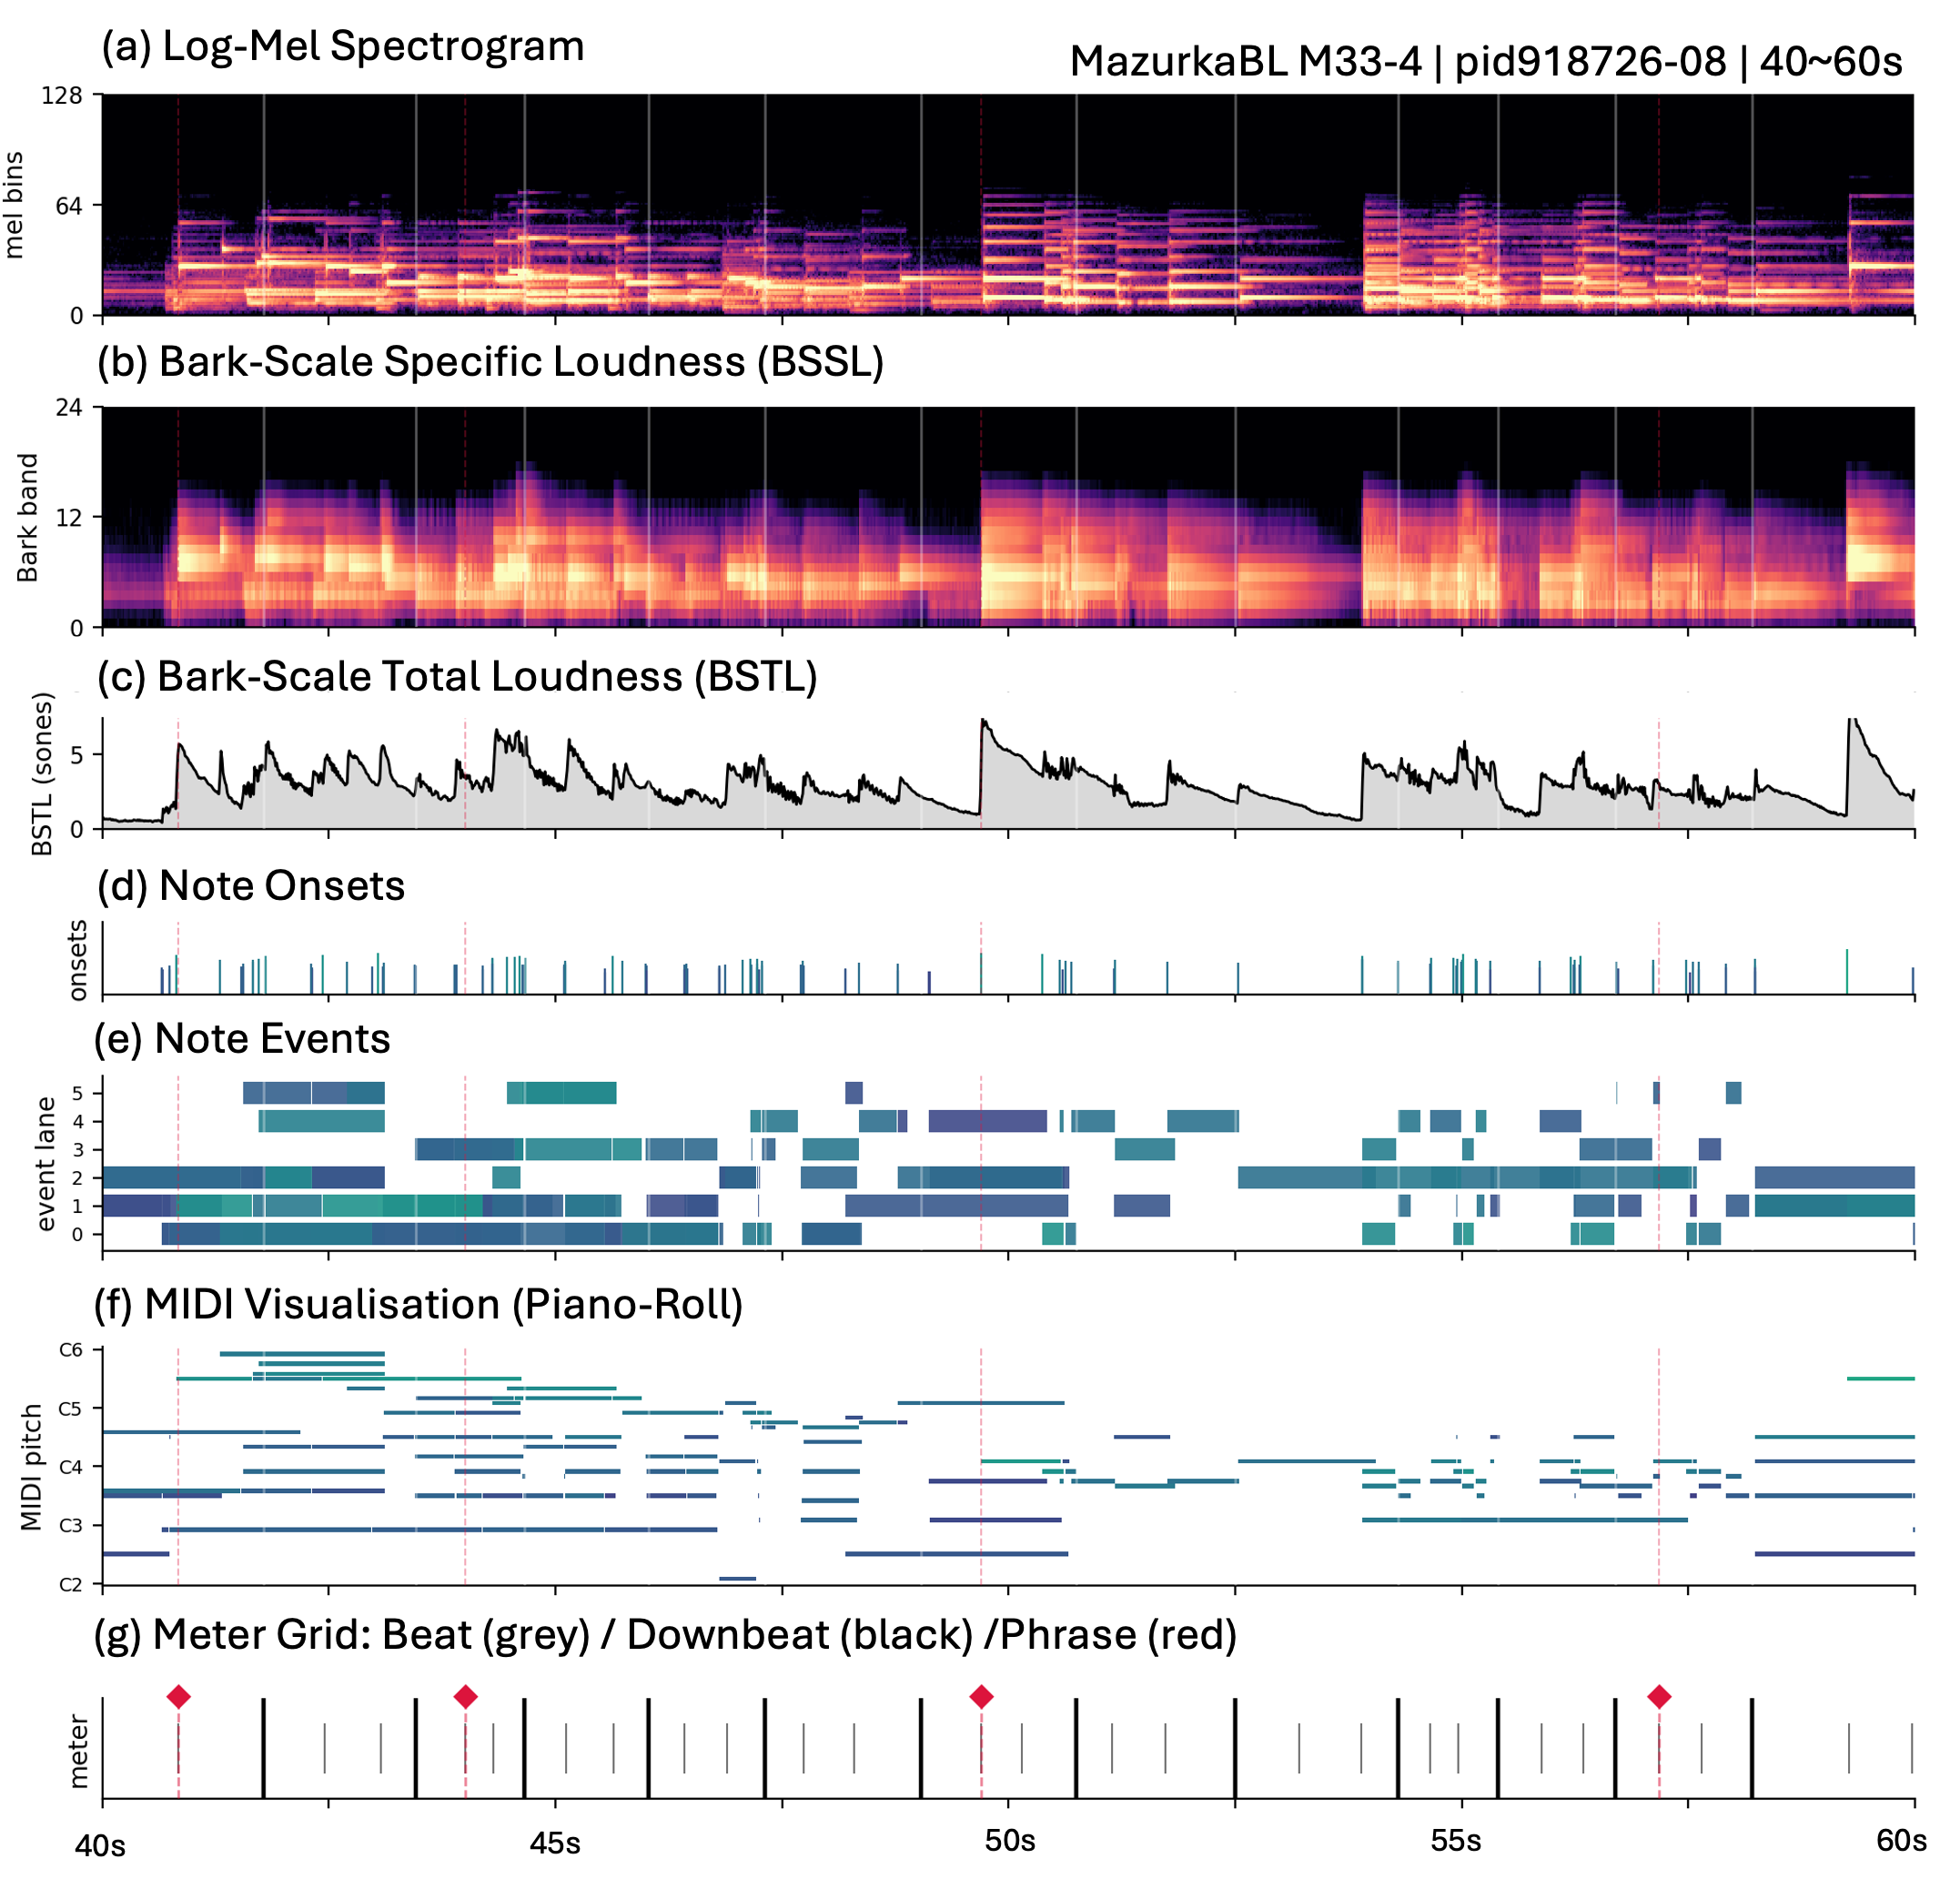
\includegraphics[width=0.98\linewidth]{Chapter_2/figures/temporal_units}
  \caption[Aligned temporal coordinates across audio, symbolic, and metrical representations]{Aligned temporal representations for a 20\,s excerpt from MazurkaBL M33-4 (pid918726-08, 40--60\,s). Panels (a)--(c) show frame-level acoustic evidence: the log-Mel spectrogram, Bark-scale specific loudness (BSSL), and Bark-scale total loudness (BSTL). Panels (d)--(f) show note-level symbolic coordinates: note onsets, note-event spans, and a MIDI piano-roll visualisation. Panel (g) shows the metrical and phrase grid, with beats in grey, downbeats in black, and phrase boundaries in red. The figure illustrates how the same performance segment can be re-indexed from dense audio frames to note events and then to beat-, bar-, and phrase-level coordinates for dynamics recovery.}
  \label{fig:bg_temporal_units}
\end{figure}


\begin{table}[!htbp]
\centering
\caption{Temporal units that recur across the thesis.}
\label{tab:bg_temporal_units}
\small
\setlength{\tabcolsep}{5pt}
\renewcommand{\arraystretch}{1.18}
\begin{tabularx}{\textwidth}{
>{\raggedright\arraybackslash}p{0.17\textwidth}
>{\raggedright\arraybackslash}p{0.34\textwidth}
>{\raggedright\arraybackslash}X
}
\toprule
\textbf{Unit} & \textbf{Where it appears} & \textbf{Why it matters} \\
\midrule
Frame & log-Mel, BSSL, BSTL, and acoustic features & Captures fine temporal evidence but is too dense for score-level dynamics \\
Note onset & MIDI velocity and AMT outputs & Natural coordinate for local attack strength and note-level intensity control \\
Note event & symbolic completion and score-informed correction & Supports note-wise masking, correction, and editable symbolic output \\
Beat & score dynamics and metrical tracking & Main coordinate for human-readable dynamic labels and beat-synchronous estimation \\
Downbeat & score dynamics and bar-level structure & Anchors metrical organisation and change-point interpretation \\
Phrase / segment & expressive interpretation and dynamic-change context & Explains longer-range shaping that cannot be reduced to isolated notes \\
\bottomrule
\end{tabularx}
\end{table}


\paragraph{Alignment.}
Alignment is not a preprocessing detail. It determines what the supervision actually means. For note-level velocity, note onsets must be aligned with either the audio or the reference score; instrumented piano corpora supply this directly through synchronised audio--MIDI capture \cite{hawthorne2019maestro}. For score dynamics, the critical coordinate is the beat grid: dynamic symbols are rarely meaningful as an unconstrained frame-wise label stream but become interpretable once mapped to beats, bars, and phrase-level change points. Figure~\ref{fig:bg_temporal_units} makes this distinction visible: the same audio frames support several possible symbolic coordinates, but only some of those coordinates match the intended target. For label-scarce settings, alignment also determines whether a proxy supervision signal (e.g.\ rendered audio reconstruction) can be compared to the observed performance at all.

\paragraph{Structural priors.}
Each task line uses a different prior to make an otherwise underdetermined dynamics target tractable. Score-informed velocity correction uses an aligned score as a structural prior over note identity (Chapter~\ref{ch:scoreinf}). Beat-synchronous score dynamics uses the metrical grid as a coordinate prior on which the label sequence lives (Chapter~\ref{ch:audiodyn}). Cross-instrument velocity recovery uses a differentiable renderer as a generative prior linking predicted control values to a measurable property of the recording (Chapter~\ref{ch:beyondpiano}). The mechanisms differ, but they share a function: they match the output layer to an evidence source and inject structure where direct supervision is weak or absent.

\section{Note-Level MIDI Velocity Recovery}
\label{sec:bg:velocity}

This section reviews the first of the three task lines: recovering note-level MIDI velocity from symbolic notes, audio, or both. It tracks the literature from rule-based humanisation through symbolic completion, audio-driven AMT, and score-informed correction, and ends at the boundary where reliable velocity supervision disappears outside piano. Chapters~\ref{ch:velcomp} and~\ref{ch:scoreinf} contribute to this line; the label-scarce extension is deferred to Section~\ref{sec:bg:synthesis}.

\subsection{Expressive rendering and humanisation}
\label{sec:bg:velocity:rendering}

Expressive performance rendering aims to generate expressive control signals from symbolic input. Many systems predict timing, dynamics, and sometimes articulation jointly \cite{jeong2019virtuosonet,borovik2023scoreperformer}. These models are important because they show that expressive performance can be learned from symbolic structure. At the same time, they reveal a practical limitation for the present thesis. Joint expressive rendering may alter more than the user wants. In production or corpus-upgrading settings, the desired operation is often narrower: preserve the notes and timing, and recover only the missing dynamics layer. This narrower, controllable objective is the entry point for Chapter~\ref{ch:velcomp}.

\subsection{Symbolic velocity completion and prediction}
\label{sec:bg:velocity:symbolic}

Symbolic velocity completion assumes that the note sequence is already known and that the missing variable is note-level velocity. Early work used rule-based or statistical approaches \cite{berndt2010modelling}. More recent work formulates the task with deep learning, including convolutional autoencoders and sequence-to-sequence models with attention \cite{kuo2021velocity,kim2023piano}. Diffusion-based note-intensity estimation has also been explored in related score-informed settings \cite{kim2023diffvel}.

A central challenge in this literature is the sparsity of symbolic piano-roll data. Dense frame grids contain large silent regions, and a model that treats all cells equally can waste much of its capacity. Two architectural patterns recur in response. The first rasterises MIDI as piano-roll-like matrices indexed by pitch and time \cite{he2025filling}, then processes them with U-Net-style encoders that preserve fine local detail through skip connections while aggregating larger context through the encoder--decoder path. The second couples this locality with windowed or linear attention to extend the receptive field without the full cost of global attention \cite{shen2023linear,chen2022hts}. Together they motivate the image-like, sparse-2D formulation adopted in Chapter~\ref{ch:velcomp}.

\subsection{Audio-driven velocity estimation within AMT}
\label{sec:bg:velocity:amt}

Velocity recovery from audio has become increasingly feasible for piano because large aligned datasets exist with sensor-recorded note velocities \cite{hawthorne2019maestro}. Representative velocity-enabled AMT systems include OaF, HPT, hFT-Trans, and event-based models \cite{hawthorne2018onsets,hawthorne2021trans,kong2021hpt,toyama2023hft,yan2021semicrf,yan2024semicrf}. Related work also studies robustness, semi-supervised learning, and parameter-efficient piano transcription \cite{maman2022general,edwards2024general,strahl2024semi,wei2022hppnet,wang2025multitask}.

Despite strong progress, note-level velocity remains more fragile than note pitch and onset estimation. The trend is already visible in Table~\ref{tab:amt_sota}: as the evaluation tightens from frame F1 to note$+$offset$+$velocity F1, the gap between leading systems widens. Domain shift in piano timbre, microphone placement, room acoustics, and recording chain degrades the mapping from acoustic evidence to velocity more severely than the mapping from acoustic evidence to pitch. This fragility is one of the main motivations for the score-informed correction strategy of Chapter~\ref{ch:scoreinf}.

\subsection{Score-informed MIDI velocity estimation and correction}
\label{sec:bg:velocity:scoreinf}

Score-informed velocity estimation assumes that an aligned score is available together with performance audio. Historically, this line of work developed partly because early AMT systems focused on notes and offered limited support for reliable velocity estimation \cite{amt2013ov}. Early systems used hand-designed measurements or parametric estimation strategies \cite{dan2006psy,goebl2003role,szeto2005finding,ewert2011est}. Later work introduced restricted Boltzmann machines, score-informed non-negative matrix factorisation, diffusion-based note-level estimation, and FiLM-conditioned deep models \cite{van2014pred,jeong2017note,jeong2018timbre,kim2023diffvel,kim2023score,kim2024method,simonetta2022acoustics}.

A key pattern in this literature is \emph{feature fusion}. Score information is injected into the acoustic model during feature extraction. This can improve accuracy, but it also ties the score-informed method tightly to a particular backbone. The present thesis instead emphasises \emph{late correction}. A correction module can attach to an existing AMT system and refine its velocity estimate while leaving the backbone largely unchanged. The natural interface for this stance is a note-token representation rather than a dense frame grid: when note events are already known, focusing modelling capacity on the events that actually require correction is more efficient than re-running a full transcription model end to end. This is the design stance developed in Chapter~\ref{ch:scoreinf}, where a score-informed Transformer over note tokens corrects a coarse velocity estimate from a frozen AMT front-end.

\subsection{Piano bias and the beyond-piano boundary}
\label{sec:bg:velocity:beyond}

Reliable velocity supervision is still strongly piano-centric. Instrumented pianos make note-level velocity available at scale, but comparable datasets for other instruments are scarce. This creates both a training bias and an evaluation bias. Transfer beyond piano must therefore confront two bottlenecks: missing labels and instrument-dependent mappings between performer action, timbre, and loudness.

The important point is that beyond-piano failure is not only ordinary domain shift. It is a measurement problem. Outside piano, even defining what a ``ground-truth'' note-level control signal should be is non-trivial: there is no sensor analogue of the Disklavier hammer trace for guitar, violin, or wind instruments. This distinction is essential for the honest positioning of Chapter~\ref{ch:beyondpiano}, and it motivates the analysis-by-synthesis route reviewed in Section~\ref{sec:bg:synthesis}.

\section{Beat-Synchronous Score-Dynamics Recovery}
\label{sec:bg:scoredyn}

This section reviews the second task line: recovering beat-anchored dynamic markings such as \textit{p}, \textit{f}, and crescendo from performance audio, together with the metrical structure on which those markings live. The output is a sparse, score-facing sequence rather than dense note-level control, and the target representation is therefore quite different from the velocity recovery reviewed in Section~\ref{sec:bg:velocity}. Chapter~\ref{ch:audiodyn} contributes to this task line.

\subsection{From performed loudness to score dynamics}
\label{sec:bg:scoredyn:loudness}

Computational modelling of dynamics has a long history in expressive performance research \cite{cancinoChacon2018computational}. Rather than focusing only on note-level control, this line of work studies how performed loudness relates to symbolic dynamic markings and phrase structure. Kosta and collaborators showed both the usefulness and the ambiguity of this relationship \cite{kosta2014dynpiano,kosta2016mapping,kosta2018mazurkabl}. Other work has further analysed dynamic principles in piano performance \cite{jones2023probingdyn}.

From a machine-learning perspective, score-dynamics recovery can be framed as classification or structured sequence labelling. The input is audio. The output is a sequence of dynamic symbols or dynamic regimes. The choice of audio representation is therefore not neutral. In the MazurkaBL line of work, the performed-loudness side of this mapping is extracted through sone-based psychoacoustic processing rather than raw amplitude, precisely because the target concerns perceived intensity rather than unweighted energy \cite{kosta2017thesis}. More generally, perceptual front-ends such as Bark-scale specific loudness preserve both a scalar loudness trajectory and the Bark-wise distribution of loudness across the spectrum, which gives a better inductive bias for loudness-oriented tasks than log-Mel features \cite{narang2024automatic,he2026dynest}. Figure~\ref{fig:bg_temporal_units}(a)--(c) shows this contrast on the same excerpt. The practical consequence is also clear: a Nyquist-constrained Bark front-end is substantially lower-dimensional than a $128$-band log-Mel representation, which enables longer audio segments and the phrase-level context that score dynamics actually requires. The challenge is that the labels themselves are sparse, relative, and musically contextual rather than physically absolute. This is one reason why a beat-synchronous formulation is more natural than direct frame-wise regression of continuous loudness.

\subsection{Change points and dynamic segmentation}
\label{sec:bg:scoredyn:changepoints}

Dynamic markings rarely behave as independent frame labels. They form local regimes that persist over spans of music, and musical meaning often lies in the transitions between those regimes. Change-point detection therefore plays an important role. It supports segmentation, interpretation, and the recovery of phrase-level dynamic structure \cite{kosta2018mazurkabl,kosta2017thesis}. The phrase markers in Figure~\ref{fig:bg_temporal_units}(g) show the kind of longer span that cannot be recovered from isolated note or frame evidence alone. In Chapter~\ref{ch:audiodyn}, change points are estimated jointly with dynamic levels so that a score-facing output includes both local states and their transitions.

\subsection{Beat and downbeat tracking as structural coordinates}
\label{sec:bg:scoredyn:metrical}

Beat and downbeat tracking has a mature literature. Early deep-learning approaches treated beats and downbeats as jointly modelled targets using recurrent neural networks combined with probabilistic post-processing such as dynamic Bayesian networks \cite{bock2016joint}, an RNN--DBN paradigm that dominated the field for several years. Subsequent work refined this combination with stronger convolutional encoders and tighter post-processing \cite{bock2020deconstruct,zhao2022beat}, while more recent Transformer-based systems further reduce reliance on heavy post-processing \cite{foscarin2024beat}. For this thesis, beat and downbeat tracking is not only a useful auxiliary task. It is the coordinate system that makes score dynamics interpretable, comparable, and writable back to a score, as reflected in the bottom grid of Figure~\ref{fig:bg_temporal_units}.

\subsection{Multi-scale and multi-task formulations}
\label{sec:bg:scoredyn:joint}

Dynamics estimation and metrical estimation are closely related but not identical, and they live at different temporal scales. Beat and downbeat tracking needs fine temporal resolution to localise peaks; phrase-level dynamics needs much longer context to read shape, contrast, and change-point structure. Multi-scale architectures address this scale mismatch by providing parallel or hierarchical pathways with different effective receptive fields \cite{li2023frame}.

The remaining issue is that even a shared multi-scale encoder can suffer from negative transfer when several tasks compete for the same representation. Multi-task learning is attractive when the outputs share information, but it is dangerous when the tasks prefer different acoustic cues. Mixture-of-experts methods provide a practical compromise: they combine shared representation learning with task-specific routing so that each output draws differently from a shared expert pool \cite{ma2018mmoe}. The MMoE-style decoder used in Chapter~\ref{ch:audiodyn} follows precisely this logic, and the combination of a perceptually grounded multi-scale encoder with task-aware routing is the architectural shape that this task line ultimately motivates.

\section{Audio Rendering and Differentiable Synthesis}
\label{sec:bg:synthesis}

This section reviews the third task line: mapping symbolic control values back to audio through a renderer, and using that mapping as supervision when direct labels are missing. The review proceeds in three steps. Section~\ref{sec:bg:synth:traditional} surveys traditional renderers and the role velocity plays inside them. Section~\ref{sec:bg:synth:diff} reviews differentiable synthesis and the design space it opens. Section~\ref{sec:bg:synth:analysis} discusses the analysis-by-synthesis paradigm and its application to label-scarce velocity recovery in Chapter~\ref{ch:beyondpiano}.

\subsection{Traditional renderers and the velocity control point}
\label{sec:bg:synth:traditional}

Traditional MIDI-to-audio rendering covers three broad families. \emph{Sample-based} synthesisers such as SoundFont-driven engines (e.g.\ FluidSynth~\cite{fluidsynth}) produce sound by selecting prerecorded samples and post-processing them with envelopes and filters; commercial samplers and free SoundFonts such as Salamander Grand Piano~\cite{sf_salamander} share this design. \emph{Physical models} such as Pianoteq~\cite{pianoteq8} replace samples with mechanical simulations of the instrument. \emph{Wavetable, FM, and additive engines} synthesise the signal from compact spectral or oscillator parameters. The three families differ in the underlying model, but they all expose MIDI velocity as a control input that drives intensity, timbral brightness, attack character, and sometimes sample-layer selection.

The implication for dynamics recovery is twofold. First, velocity is not a renderer-independent loudness unit: the same MIDI velocity can produce substantially different acoustic outputs depending on which sample layers, envelopes, or physical parameters the renderer uses, as already discussed in Section~\ref{sec:bg:dynamics_midi_score}. Figures~\ref{fig:bg_instruments_sone} and~\ref{fig:bg_instruments_guitar} make this concrete by showing how the velocity-to-loudness response curves of representative SoundFonts differ within the piano family and across instruments. Second, traditional renderers are not differentiable: they expose discrete sample selection, table lookups, and non-smooth envelopes, so gradients cannot flow from rendered audio back to the velocity input. Any system that wants to use rendering as a learning signal must therefore replace, approximate, or wrap the renderer with a differentiable proxy.

\begin{figure}[!htbp]
  \centering
  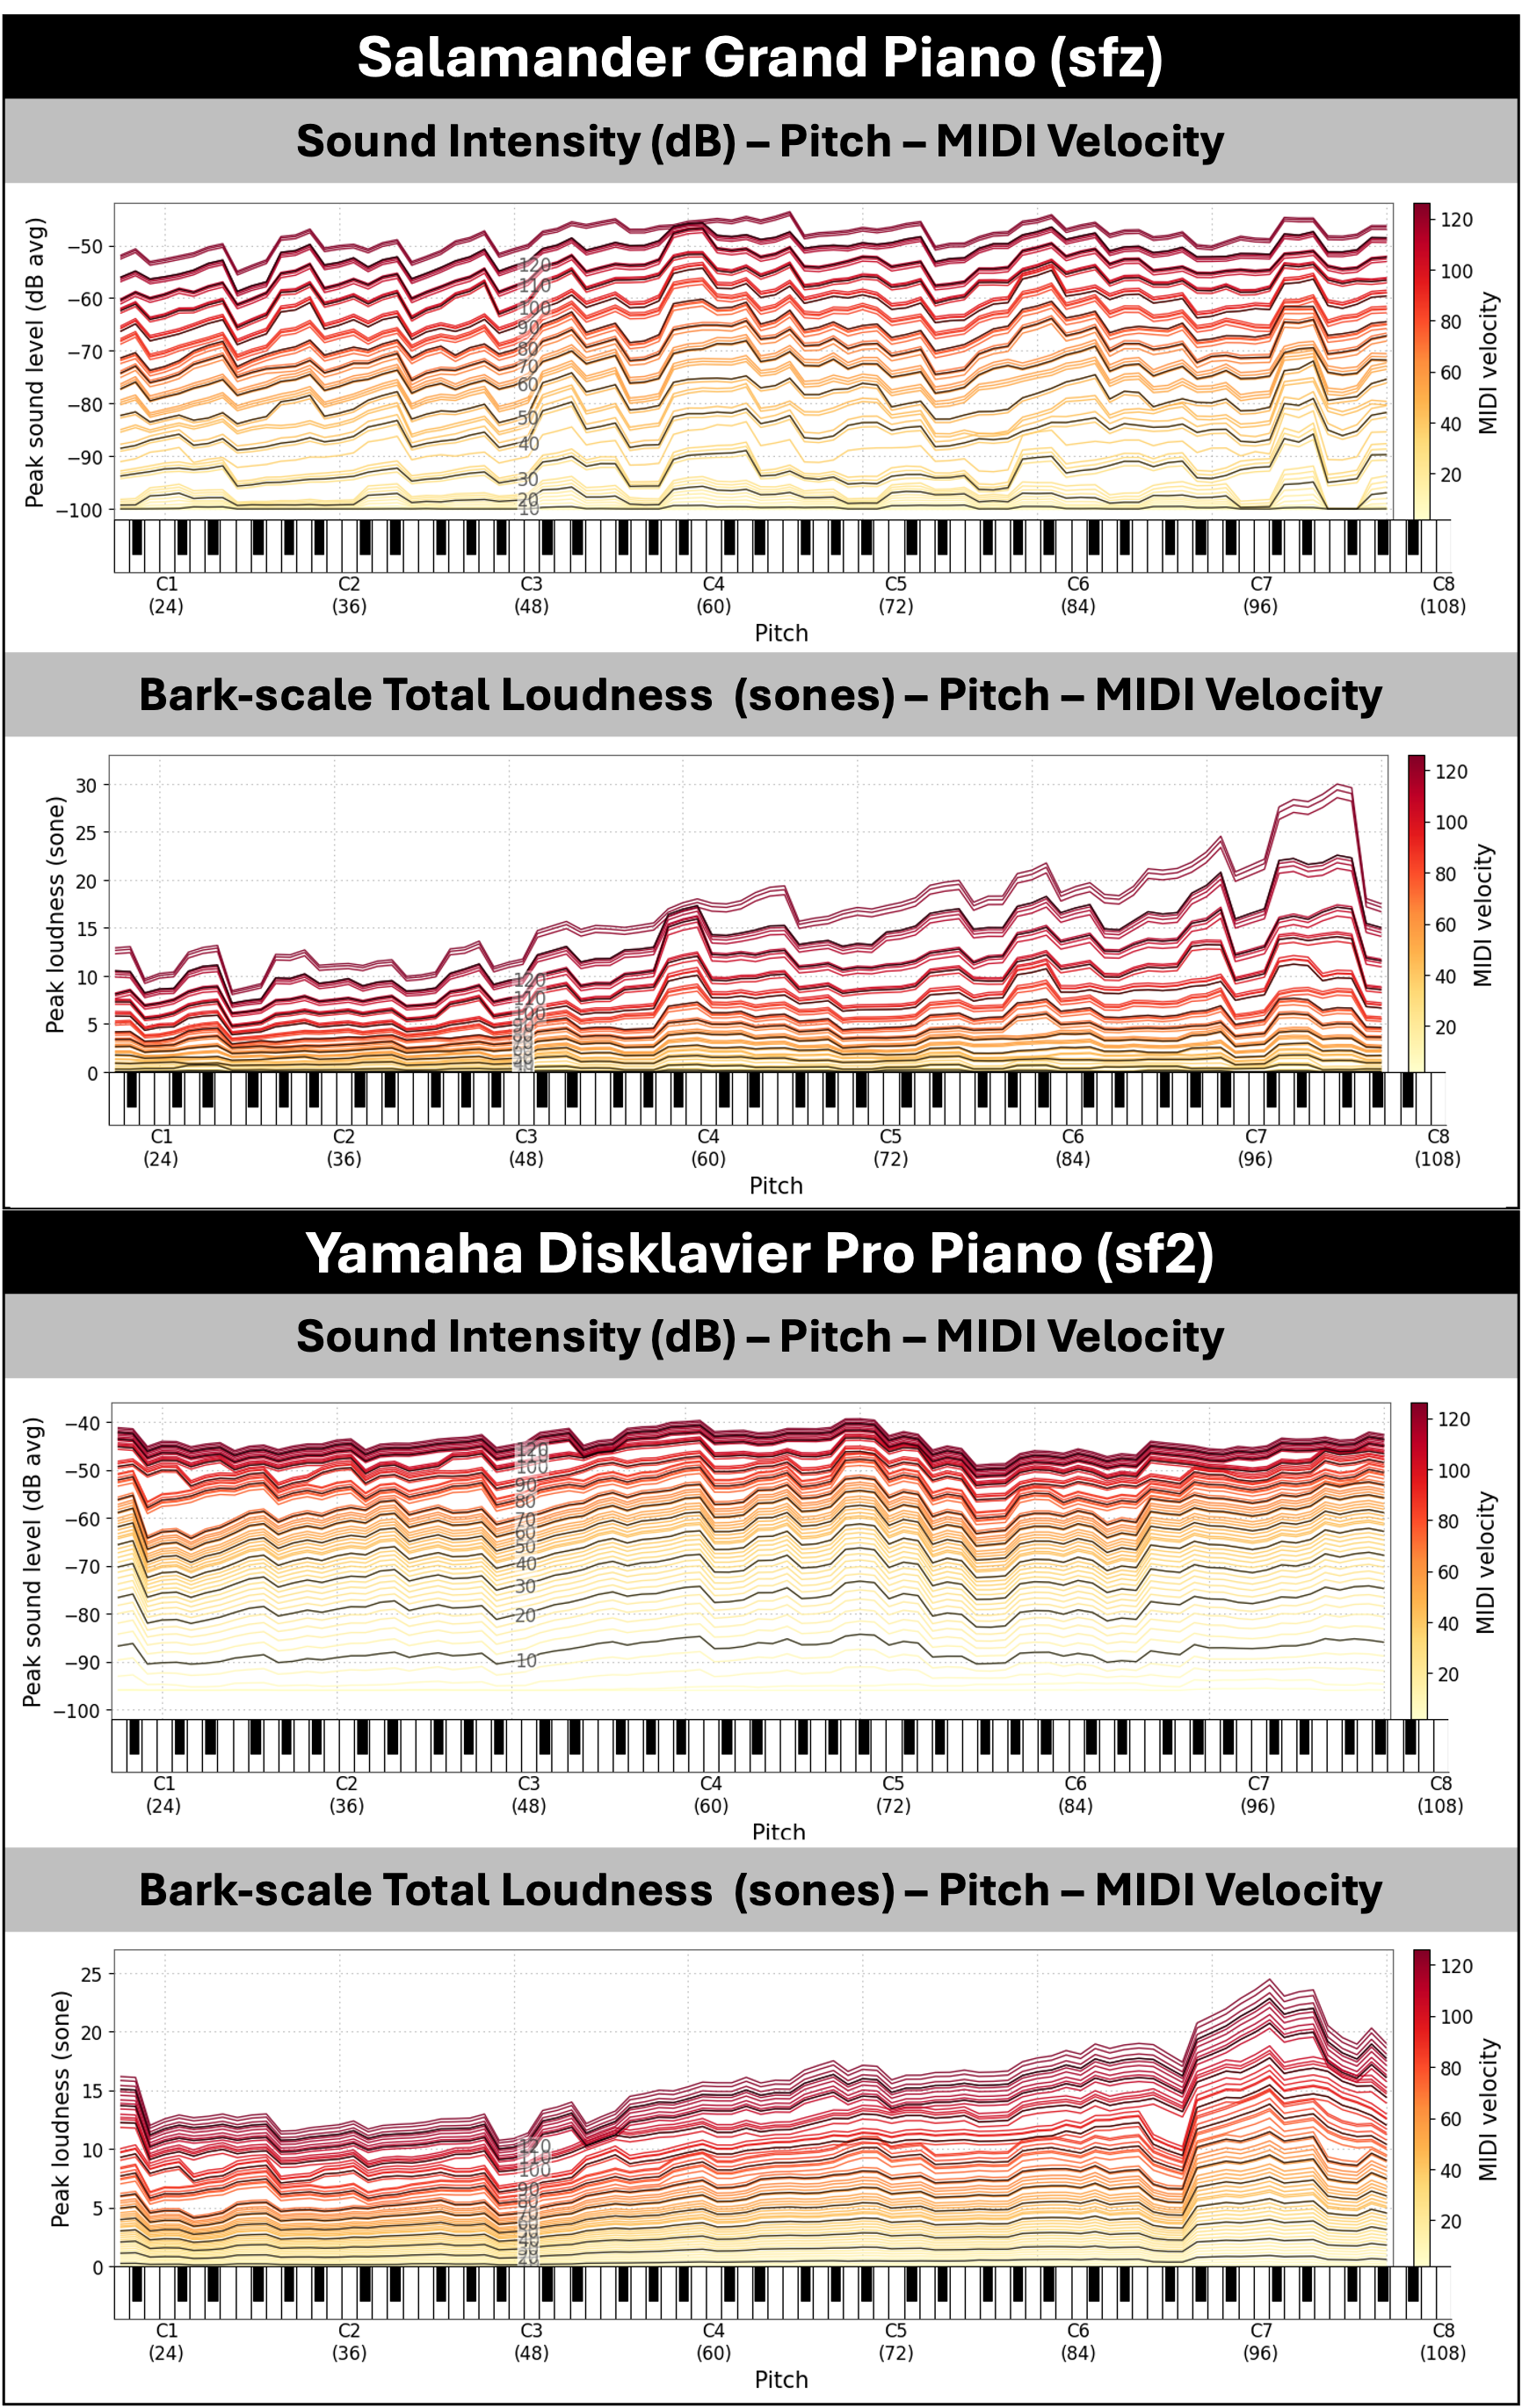
\includegraphics[width=0.9\linewidth]{Chapter_2/figures/soundfont_piano.png}
  \caption{Velocity-to-loudness response of two piano renderers (Salamander Grand Piano and a Yamaha Disklavier Pro SoundFont). Both share the same input control range, but the realised loudness curves differ in slope and shape, which illustrates the renderer dependence of MIDI velocity.}
  \label{fig:bg_instruments_sone}
\end{figure}

\begin{figure}[!htbp]
  \centering
  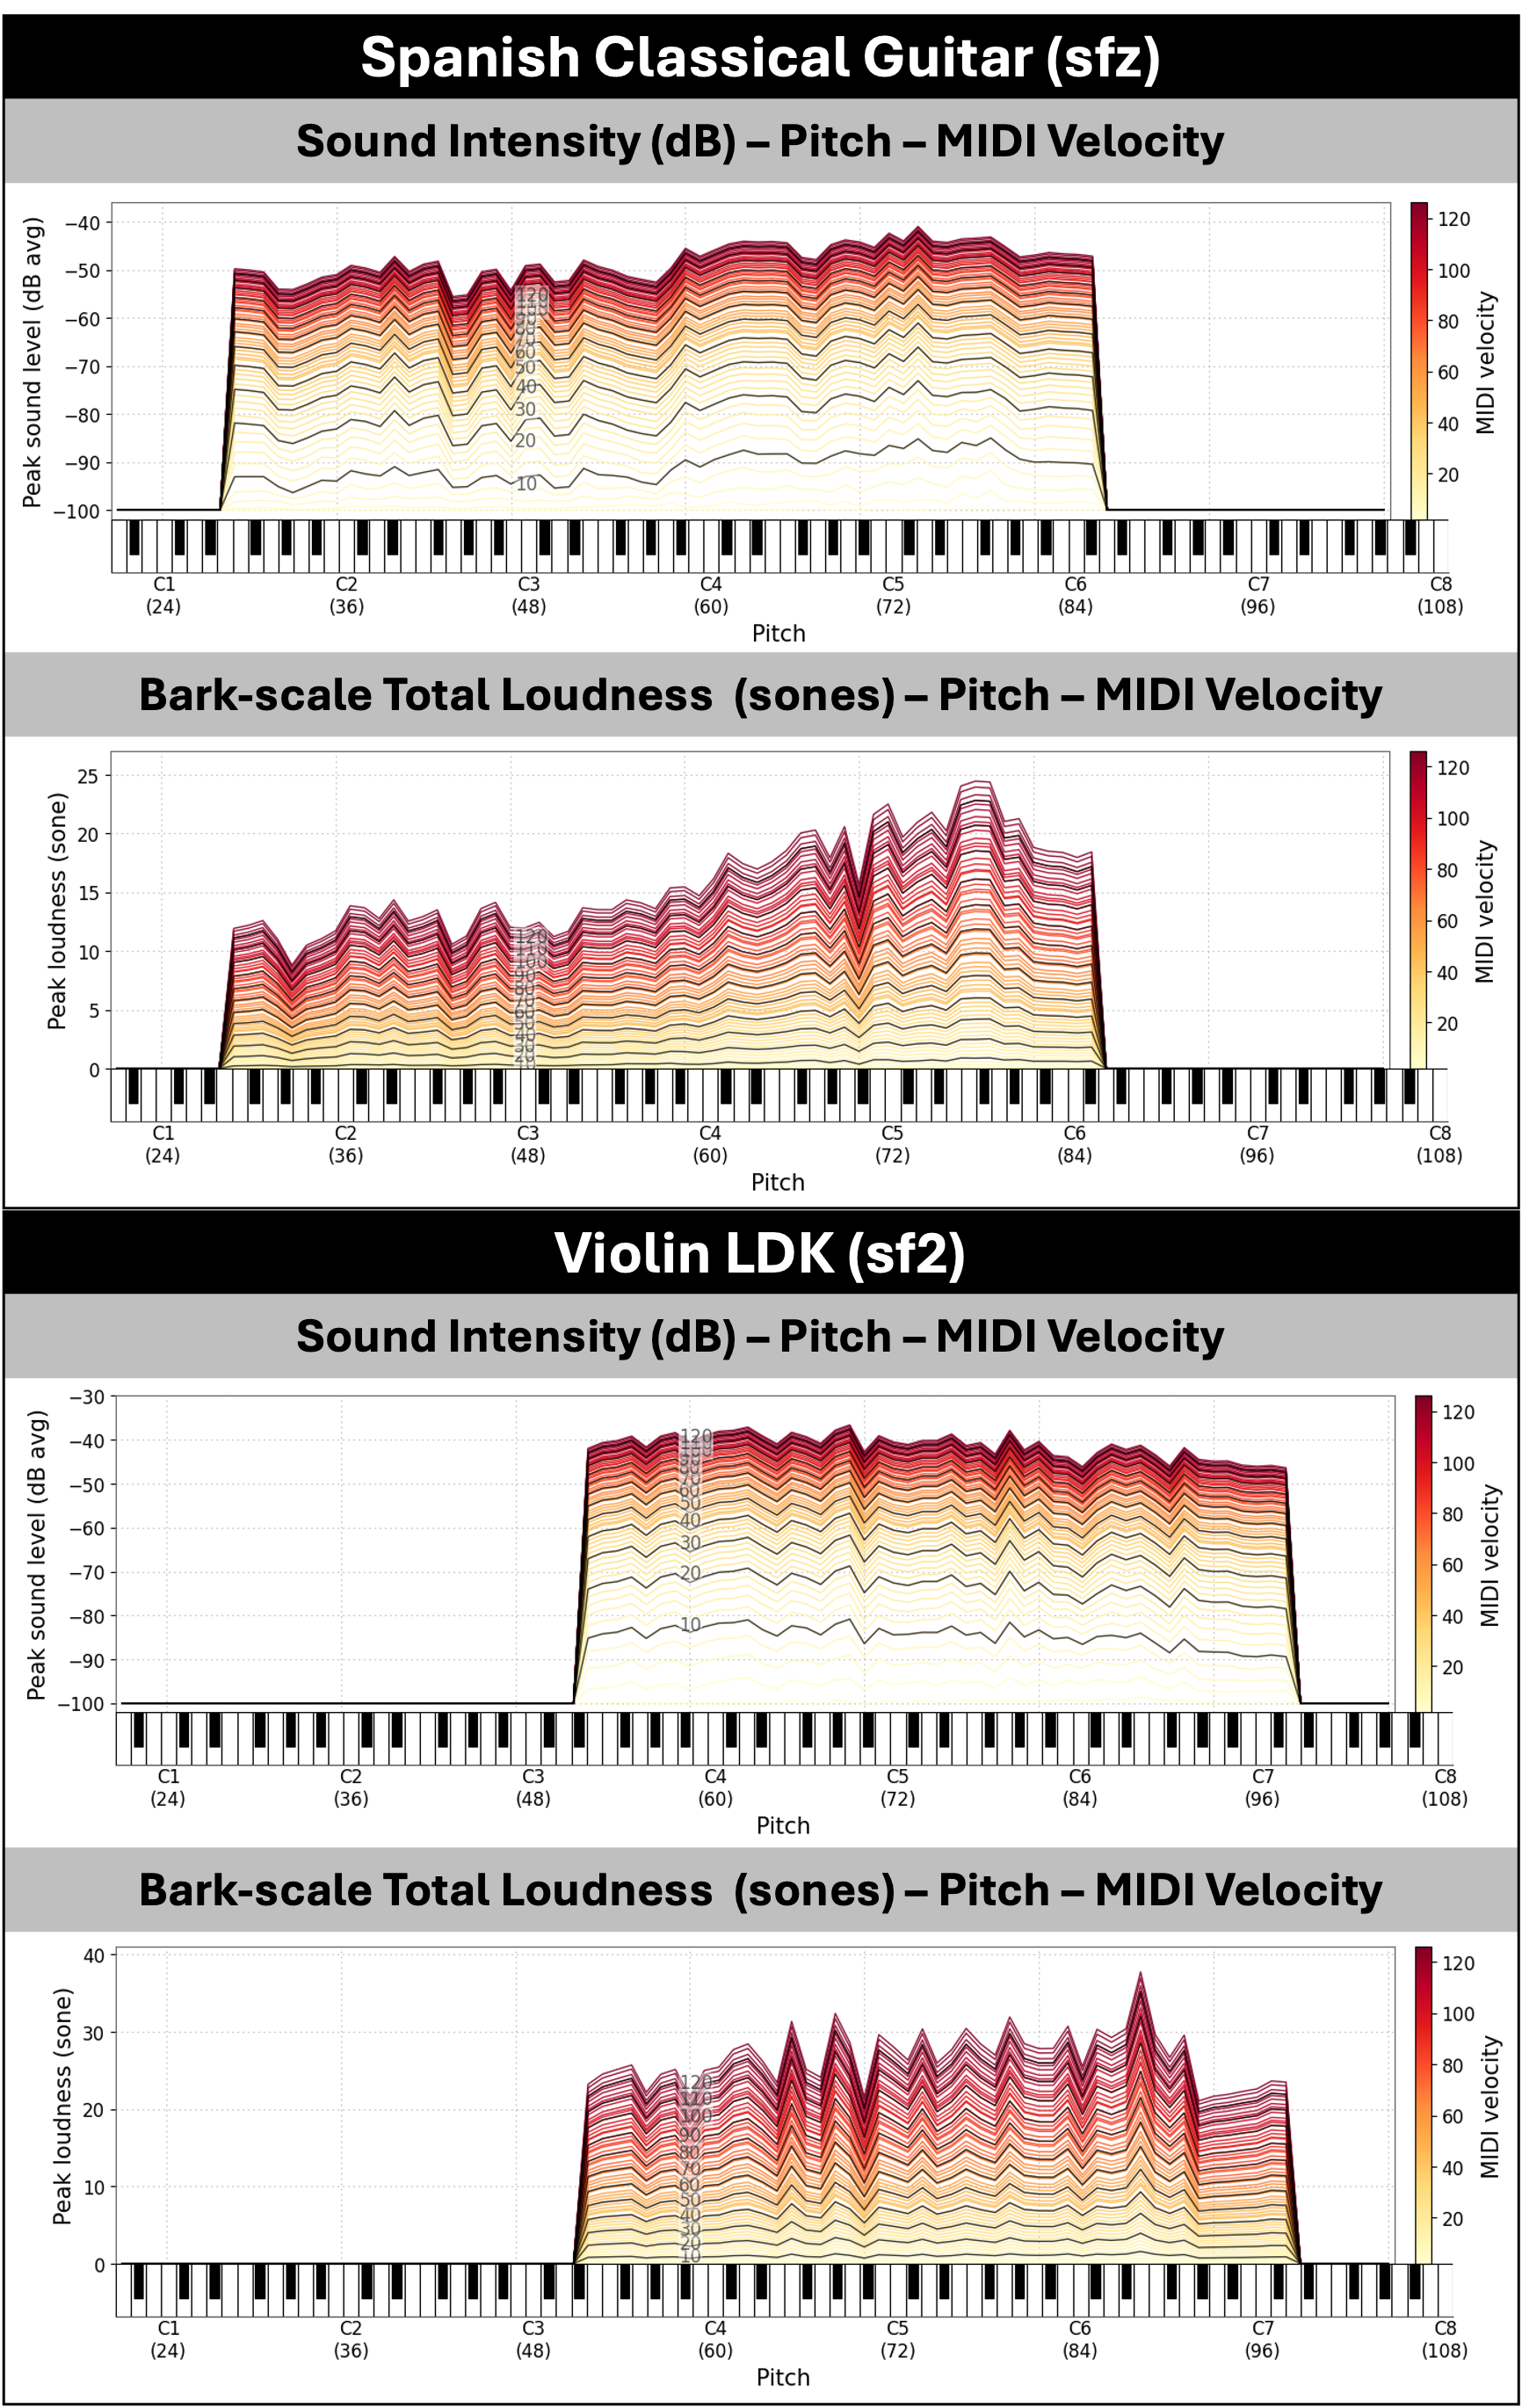
\includegraphics[width=0.9\linewidth]{Chapter_2/figures/soundfont_guitar.png}
  \caption{Velocity-to-loudness response for non-piano SoundFonts (Spanish Classical Guitar and Violin LDK). Compared with Figure~\ref{fig:bg_instruments_sone}, the curves show different dynamic ranges and saturation behaviour, motivating the need for a renderer-aware supervision interface when working beyond piano.}
  \label{fig:bg_instruments_guitar}
\end{figure}

\subsection{Differentiable synthesis}
\label{sec:bg:synth:diff}

Differentiable synthesis was introduced to make audio rendering compatible with gradient-based learning. The DDSP framework expresses a renderer as a small differentiable graph (harmonic-plus-noise oscillators, time-varying filters) whose control signals are predicted by a neural network~\cite{engel2020ddsp,hayes2024ddsp_review}. Loss functions are then applied in the signal or spectral domain, and gradients flow back through the renderer to the network. The same idea has been adapted to specific instruments and rendering goals: MIDI-DDSP couples DDSP with explicit note-level control for expressive performance synthesis~\cite{wu2022mididdsp}, DDSP-Piano specialises the framework to piano timbre with mechanically motivated components~\cite{renault2023ddsp_piano}, and follow-up work extends it to acoustic guitar and other plucked-string instruments~\cite{wiggins2023ddsp_guitar_model,jonason2024guitar}. Beyond DDSP, differentiable approximations to traditional samplers and effects processors have been studied as well~\cite{martinez2021differentiable,shan2022differentiable,simionato2025neuralsample}, and recent work has explored normalising-flow and transformer-based generative renderers in similar settings~\cite{yang2026flowsynth,zang2024synthtab}.

For dynamics recovery, the appeal is direct. A differentiable renderer turns the velocity-to-audio mapping into a learnable layer. A model can predict velocity, render the resulting audio, and back-propagate a reconstruction error. This makes velocity-relevant supervision possible even when direct note-level labels are absent. The cost is also direct: differentiable renderers are not free reproductions of every commercial synthesiser. They tend to specialise to one instrument family, and their fidelity to real recordings depends on how much of the timbral, recording-chain, and room behaviour the renderer captures. The choice of differentiable renderer therefore conditions what the downstream model can plausibly learn.

\subsection{Analysis-by-synthesis and label-scarce velocity recovery}
\label{sec:bg:synth:analysis}

The combination of differentiable rendering and prediction networks defines an \emph{analysis-by-synthesis} setting. A network proposes control values for an observed recording; the renderer turns those values back into audio (or into an intermediate audio-derived quantity); a loss compares the rendered output with the observed signal. This paradigm becomes the central tool when true note-level velocity labels are unavailable, because the renderer takes the place of a label by linking predicted control to a measurable property of the recording.

Two design axes matter for this thesis. The first is the comparison space. \emph{Signal-domain} losses (waveform or spectral) can be applied directly to the rendered output, but they conflate velocity with timbre, recording chain, and room response, so the gradient signal is dominated by factors unrelated to velocity. \emph{Parameter-domain} or perceptual proxy losses instead extract a small set of velocity-relevant acoustic descriptors (e.g.\ note-wise loudness, attack envelope) from both the rendered and the observed audio and compare them in that lower-dimensional space. The latter is closer in spirit to the parameter-extraction proxies used in spectral-modelling research and trades waveform fidelity for stronger alignment with the velocity target. The second axis is the renderer's domain coverage. A differentiable renderer adapted to piano need not transfer to guitar or violin without further work~\cite{renault2023ddsp_piano,wiggins2023ddsp_guitar_model}, which is one of the practical constraints of cross-instrument analysis-by-synthesis.

For expressive AMT, this strategy is attractive but delicate. It makes label-scarce learning possible, yet it also ties the learning signal to the adequacy of the renderer: a proxy objective can reward compatibility with the synthesiser more than compatibility with real instrumental control, and reconstruction error is therefore not the same thing as accurate velocity recovery. Chapter~\ref{ch:beyondpiano} adopts the analysis-by-synthesis route explicitly under these constraints. It contrasts a waveform-domain DDSP-style supervision interface with a low-dimensional parameter-space proxy built from a frozen SoundFont teacher, and treats proxy supervision as a method family with explicit limits rather than as a universal substitute for true note-level labels.

\section{Datasets, Evaluation, and Reproducibility Constraints}
\label{sec:bg:dataeval}

The empirical claims of this thesis are conditioned on what each available dataset can support. Table~\ref{tab:dataset_comparison} summarises the representative corpora relevant to expressive label recovery, listing their instrument coverage, scale, and which expressive modalities (MIDI velocity, score, and score dynamics) are actually available. The discussion that follows turns these modality differences into chapter-specific constraints.

\begin{table}[!htbp]
\centering
\caption{Representative datasets relevant to expressive label recovery in this thesis. Each dataset is summarised by its instrument family, scale, and the expressive modalities (MIDI, velocity, score, score dynamics) it provides.}
\label{tab:dataset_comparison}

\setlength{\tabcolsep}{2.4pt}
\fontsize{11pt}{11pt}\selectfont
\renewcommand{\arraystretch}{1.2}

\begin{tabularx}{\textwidth}{
l l
c c c
c c c c
}
\toprule
\multirow{2}{*}{\textbf{Dataset}} &
\multirow{2}{*}{\textbf{Instr.}} &
\multicolumn{3}{c}{\textbf{Statistic}} &
\multicolumn{4}{c}{\textbf{Modality}} \\
\cmidrule(lr){3-5} \cmidrule(lr){6-9}
&
& \textbf{Hours}
& \makecell{\textbf{Perfor-}\\\textbf{mance}}
& \makecell{\textbf{Compos-}\\\textbf{itions}}
& \textbf{MIDI}
& \makecell{\textbf{Velocity}}
& \textbf{Score}
& \makecell{\textbf{Dynamics}} \\
\midrule

\addlinespace[2pt]
ATEPP \cite{zhang2022atepp}
& piano
& 1007
& 11742
& 1580
& \cmark
& \cmark
& \cmark\ 43\%
& \warn\ 43\% \\
\addlinespace[4pt]
\multicolumn{9}{>{\raggedright\arraybackslash}p{\dimexpr\textwidth-2\tabcolsep\relax}}
{\hspace{1em}\warn\ Audio is from YouTube (availability may vary); score dynamics are not verified.} \\
\addlinespace[2pt]
\midrule

\addlinespace[2pt]
ASAP \cite{foscarin2020asap}
& piano
& 92
& 1068
& 222
& \cmark
& \cmark
& \cmark
& \warn \\
\addlinespace[4pt]
\multicolumn{9}{>{\raggedright\arraybackslash}p{\dimexpr\textwidth-2\tabcolsep\relax}}
{\hspace{1em}\warn\ Score dynamics (and other expressive markings) are not verified.} \\
\addlinespace[2pt]
\midrule

\addlinespace[2pt]
MAESTRO v3 \cite{hawthorne2019maestro}
& piano
& 172
& 1276
& 864
& \cmark
& \cmark
& \xmark
& \xmark \\
\addlinespace[4pt]
\multicolumn{9}{>{\raggedright\arraybackslash}p{\dimexpr\textwidth-2\tabcolsep\relax}}
{\hspace{1em}\cmark\ High-quality piano dataset, recorded on Yamaha Disklavier pianos.} \\
\addlinespace[2pt]
\midrule

\addlinespace[2pt]
SMD v2 \cite{smd}
& piano
& 4.7
& 50
& 50
& \cmark
& \cmark
& \xmark
& \xmark \\
\addlinespace[4pt]
\multicolumn{9}{>{\raggedright\arraybackslash}p{\dimexpr\textwidth-2\tabcolsep\relax}}
{\hspace{1em}\cmark\ Often used for cross-dataset evaluation; recorded on Yamaha Disklavier pianos.} \\
\addlinespace[2pt]
\midrule

\addlinespace[2pt]
MAPS \cite{maps}
& piano$^\dagger$ 
& 17.9
& 270
& 208
& \cmark
& \cmark
& \xmark
& \xmark \\
\addlinespace[4pt]
\multicolumn{9}{>{\raggedright\arraybackslash}p{\dimexpr\textwidth-2\tabcolsep\relax}}
{\hspace{1em} \cmark Count only ENSTDkAm and ENSTDkCl subsets (solo piano, Yamaha Disklavier).} \\
\addlinespace[2pt]
\midrule

\addlinespace[2pt]
MazurkaBL \cite{kosta2018mazurkabl}
& piano
& 110
& 2000
& 44
& \xmark
& \xmark
& \cmark
& \cmark \\
\addlinespace[4pt]
\multicolumn{9}{>{\raggedright\arraybackslash}p{\dimexpr\textwidth-2\tabcolsep\relax}}
{\hspace{1em}\cmark\ Dynamics and Expressive labels are explicitly verified. All Chopin compositions.}\\
\addlinespace[2pt]
\midrule

\addlinespace[2pt]
Vienna4x22 \cite{goebl1999vienna4x22}
& piano
& 2.3
& 88
& 4
& \cmark
& \cmark
& \cmark
& \cmark \\
\addlinespace[4pt]
\multicolumn{9}{>{\raggedright\arraybackslash}p{\dimexpr\textwidth-2\tabcolsep\relax}}
{\hspace{1em}\cmark Contains 4 compositions from Chopin, Schubert and Mozart, each 22 performances.} \\
\addlinespace[2pt]
\midrule

\addlinespace[2pt]
Batik-plays-Mozart~\cite{hu2023batik}
& piano
& 3.7
& 36
& 36
& \cmark
& \cmark
& \cmark
& \cmark \\
\addlinespace[4pt]
\multicolumn{9}{>{\raggedright\arraybackslash}p{\dimexpr\textwidth-2\tabcolsep\relax}}
{\hspace{1em}\cmark Contains 12 Mozart sonatas split to 36 movement-level score--performance pairs.} \\
\addlinespace[2pt]
\midrule

% \addlinespace[2pt]
% MSMD \cite{dorfer2018msmd}
% & piano
% & 15
% & 479
% & 479
% & \cmark
% & \xmark
% & \cmark
% & \xmark \\
% \addlinespace[4pt]
% \multicolumn{9}{>{\raggedright\arraybackslash}p{\dimexpr\textwidth-2\tabcolsep\relax}}
% {\hspace{1em}\warn\ Synthesised audio; MIDI is derived from digital scores rather than human performance.} \\
% \addlinespace[2pt]
% \midrule

\addlinespace[2pt]
GuitarSet \cite{xi2018guitarset}
& guitar
& 3.0
& 360
& 30
& \cmark
& \xmark
& \xmark
& \xmark \\
\addlinespace[4pt]
\multicolumn{9}{>{\raggedright\arraybackslash}p{\dimexpr\textwidth-2\tabcolsep\relax}}
{\hspace{1em}\cmark\ Good quality electric guitar dataset.} \\
\addlinespace[2pt]
\midrule

\addlinespace[2pt]
GOAT \cite{loth2025goat}
& guitar
& 5.9
& 172
& n/a.
& \cmark
& \xmark
& \cmark
& \xmark \\
\addlinespace[4pt]
\multicolumn{9}{>{\raggedright\arraybackslash}p{\dimexpr\textwidth-2\tabcolsep\relax}}
{\hspace{1em}\cmark\ Usage may still be constrained by copyright or redistribution terms.} \\
\addlinespace[2pt]
\midrule

\addlinespace[2pt]
Fran\c{c}ois Leduc \cite{riley2024high}
& guitar
& 4.0
& 78
& n/a.
& \cmark
& \xmark
& \warn
& \xmark \\
\addlinespace[4pt]
\multicolumn{9}{>{\raggedright\arraybackslash}p{\dimexpr\textwidth-2\tabcolsep\relax}}
{\hspace{1em}\cmark\ By request only; released files include audio--MIDI pairs, but not the original scores.} \\
\addlinespace[2pt]
\midrule

\addlinespace[2pt]
GAPS \cite{riley2024gaps}
& guitar
& 14.1
& 300
& 300
& \cmark
& \xmark
& \cmark
& \xmark \\
\addlinespace[4pt]
\multicolumn{9}{>{\raggedright\arraybackslash}p{\dimexpr\textwidth-2\tabcolsep\relax}}
{\hspace{1em}\warn\ Audio is collected from YouTube URLs (availability may vary).} \\
\addlinespace[2pt]
\midrule

\addlinespace[2pt]
MusicNet \cite{thickstun2017musicnet}
& ensemble
& 34.1
& 330
& 121
& \cmark
& \warn
& \xmark
& \xmark \\
\addlinespace[4pt]
\multicolumn{9}{>{\raggedright\arraybackslash}p{\dimexpr\textwidth-2\tabcolsep\relax}}
{\hspace{1em}\warn\ Classical, multi-instrument; velocity is score-derived and not performance control.} \\
\addlinespace[2pt]
\midrule

\addlinespace[2pt]
MID-FiLD \cite{ryu2024midfild}
& ensemble
& n/a.
& 4477
& 4477
& \cmark
& \cmark
& \xmark
& \xmark \\
\addlinespace[4pt]
\multicolumn{9}{>{\raggedright\arraybackslash}p{\dimexpr\textwidth-2\tabcolsep\relax}}
{\hspace{1em}\warn\ No human audio; MIDI is made by software rather than human performance.} \\
\addlinespace[2pt]

\bottomrule
\end{tabularx}
\end{table}

\subsection{Dataset modalities and what each chapter can learn}
\label{sec:bg:dataeval:modalities}

The thesis relies on datasets with very different modality combinations. Audio--MIDI datasets such as MAESTRO support supervised note-level velocity learning. Cross-dataset piano corpora such as SMD and MAPS stress generalisation under changed recording conditions. Score-aligned corpora such as MazurkaBL support score-facing dynamics research because they provide beat-level structure and expressive annotations. Other datasets are valuable but incomplete for the present thesis because they may lack reliable note-level velocity, verified score dynamics, or stable redistribution conditions.

These modality differences are not an implementation detail. They determine which claim can be made at all. Chapter~\ref{ch:velcomp} needs reliable symbolic velocity targets. Chapter~\ref{ch:scoreinf} additionally needs an aligned score. Chapter~\ref{ch:audiodyn} needs score-facing dynamics with metrical structure. Chapter~\ref{ch:beyondpiano} needs candidate non-piano corpora, but cannot assume direct velocity supervision of MAESTRO quality.

\subsection{Evaluation for MIDI velocity}
\label{sec:bg:dataeval:velocity}

Velocity should be evaluated at note level rather than by naive frame-wise error. Otherwise, long sustained notes dominate the metric. Standard statistics include mean absolute error and related dispersion measures \cite{kuo2021velocity,kim2024method}. However, numerical accuracy alone is not sufficient. A model can achieve a decent average error while producing over-smoothed or mechanically centred dynamics. Distribution-sensitive measures, visual inspection, and listening tests therefore play an important complementary role. This is especially evident in Chapter~\ref{ch:velcomp}, where perceptual differences are not always fully captured by raw error.

Cross-dataset evaluation is also essential. Piano type, velocity calibration, microphone placement, and room acoustics all affect the mapping from performance action to recorded signal. A model that performs well only on the training dataset does not yet solve expressive AMT in a practical sense.

\subsection{Evaluation for score dynamics}
\label{sec:bg:dataeval:scoredyn}

Score dynamics is usually evaluated as classification on a musically meaningful grid. F1 score is common because the class distribution is imbalanced and because some symbols occur much less frequently than others \cite{kosta2017thesis}. In the present thesis, beat-synchronous evaluation is especially important because it avoids arbitrary frame-level tolerance choices and aligns the prediction target with how the annotations are actually used in music notation.

Evaluation remains inherently limited by label ambiguity. Different editors or annotators may disagree on dynamic markings. Different editions of the same piece may contain different expressive symbols. This does not invalidate the task, but it does mean that score-dynamics performance must be interpreted with awareness of the annotation convention behind the dataset.

\subsection{Evaluation under proxy supervision}
\label{sec:bg:dataeval:proxy}

When direct note-level velocity labels are absent, evaluation becomes weaker and must be stated more carefully. Audio reconstruction error after differentiable synthesis is informative, but it is not equivalent to accurate velocity recovery. A proxy-supervised study should therefore separate three questions. Does the synthesised audio become more plausible? Do the predicted control values display musically reasonable distributions and relative trends? Does any anchor subset with stronger labels show positive transfer?

This evaluation logic is directly relevant to Chapter~\ref{ch:beyondpiano}. The contribution of that chapter is exploratory because the supervision and evaluation are weaker than in the piano chapters. Making that weakness explicit strengthens the thesis. It does not weaken it.

\subsection{Reproducibility, alignment quality, and licensing}
\label{sec:bg:dataeval:repro}

Expressive AMT research is strongly constrained by data quality and licensing. Many scores are copyrighted. Many recordings cannot be redistributed freely. Some datasets rely on external URLs or derived alignments whose long-term availability is uncertain. Alignment quality is another major factor. A method may fail not because the dynamics model is poor, but because the score or beat alignment is noisy.

For this reason, reproducible expressive AMT research should document preprocessing, alignment assumptions, train/validation/test protocols, and all modality constraints clearly. The later thesis chapters follow this principle, and the final conclusion of the dissertation treats these constraints as design considerations rather than afterthoughts.

\section{Summary of Gaps and Thesis Requirements}
\label{sec:bg:summary}

The review above leaves six requirements for a thesis on dynamics recovery. 

\begin{itemize}
    \item \textbf{R1 Preserve note content and timing while recovering dynamics.} Many expressive systems modify several performance dimensions jointly. The present thesis instead treats dynamics as a refinement or annotation layer. This requirement is most visible in Chapters~\ref{ch:velcomp}, \ref{ch:scoreinf}, and~\ref{ch:beyondpiano}.

    \item \textbf{R2 Support heterogeneous data-availability settings.} Real corpora differ widely in what is available: symbolic MIDI only, audio plus aligned score, audio only, or audio with only proxy supervision. This requirement motivates the overall design of Chapters~\ref{ch:velcomp}--\ref{ch:beyondpiano}.

    \item \textbf{R3 Respect representation differences explicitly.} Loudness, MIDI velocity, and score dynamics are linked but not identical. The target representation must therefore be chosen deliberately and defended in each chapter. This requirement spans the whole thesis.

    \item \textbf{R4 Use musically meaningful coordinates for score-level outputs.} Score dynamics should not be treated as an arbitrary frame-wise label stream. It should be expressed on a beat-synchronous interface, supported by downbeat and phrase-level context, that supports interpretation, evaluation, and symbolic writing. This requirement motivates Chapter~\ref{ch:audiodyn}.

    \item \textbf{R5 Evaluate with both numerical and musical evidence.} Objective metrics are necessary but not always sufficient. Listening tests, qualitative inspection, distributional behaviour, and cross-dataset evaluation remain important. This requirement is visible in Chapters~\ref{ch:velcomp}, \ref{ch:audiodyn}, and~\ref{ch:beyondpiano}.

    \item \textbf{R6 Treat beyond-piano transfer as a supervision problem rather than ordinary domain shift.} Once true note-level velocity labels disappear, the central issue is no longer only acoustic domain mismatch, but the absence of a directly measurable target. This requirement motivates Chapter~\ref{ch:beyondpiano}, where proxy supervision is formulated as a renderer-conditioned route to label-scarce velocity recovery.
\end{itemize}

These requirements define the dissertation stance. Dynamics recovery is treated as controlled label restoration under structural preservation, not as unconstrained expressive generation. The four technical chapters instantiate this stance under progressively weaker or different evidence conditions: symbolic-only completion, score-informed audio refinement, audio-only score-dynamics recovery, and renderer-conditioned recovery when target-domain velocity labels are absent.